\documentclass[twoside]{book}

% Packages required by doxygen
\usepackage{fixltx2e}
\usepackage{calc}
\usepackage{doxygen}
\usepackage[export]{adjustbox} % also loads graphicx
\usepackage{graphicx}
\usepackage[utf8]{inputenc}
\usepackage{makeidx}
\usepackage{multicol}
\usepackage{multirow}
\PassOptionsToPackage{warn}{textcomp}
\usepackage{textcomp}
\usepackage[nointegrals]{wasysym}
\usepackage[table]{xcolor}

% Font selection
\usepackage[T1]{fontenc}
\usepackage[scaled=.90]{helvet}
\usepackage{courier}
\usepackage{amssymb}
\usepackage{sectsty}
\renewcommand{\familydefault}{\sfdefault}
\allsectionsfont{%
  \fontseries{bc}\selectfont%
  \color{darkgray}%
}
\renewcommand{\DoxyLabelFont}{%
  \fontseries{bc}\selectfont%
  \color{darkgray}%
}
\newcommand{\+}{\discretionary{\mbox{\scriptsize$\hookleftarrow$}}{}{}}

% Page & text layout
\usepackage{geometry}
\geometry{%
  a4paper,%
  top=2.5cm,%
  bottom=2.5cm,%
  left=2.5cm,%
  right=2.5cm%
}
\tolerance=750
\hfuzz=15pt
\hbadness=750
\setlength{\emergencystretch}{15pt}
\setlength{\parindent}{0cm}
\setlength{\parskip}{3ex plus 2ex minus 2ex}
\makeatletter
\renewcommand{\paragraph}{%
  \@startsection{paragraph}{4}{0ex}{-1.0ex}{1.0ex}{%
    \normalfont\normalsize\bfseries\SS@parafont%
  }%
}
\renewcommand{\subparagraph}{%
  \@startsection{subparagraph}{5}{0ex}{-1.0ex}{1.0ex}{%
    \normalfont\normalsize\bfseries\SS@subparafont%
  }%
}
\makeatother

% Headers & footers
\usepackage{fancyhdr}
\pagestyle{fancyplain}
\fancyhead[LE]{\fancyplain{}{\bfseries\thepage}}
\fancyhead[CE]{\fancyplain{}{}}
\fancyhead[RE]{\fancyplain{}{\bfseries\leftmark}}
\fancyhead[LO]{\fancyplain{}{\bfseries\rightmark}}
\fancyhead[CO]{\fancyplain{}{}}
\fancyhead[RO]{\fancyplain{}{\bfseries\thepage}}
\fancyfoot[LE]{\fancyplain{}{}}
\fancyfoot[CE]{\fancyplain{}{}}
\fancyfoot[RE]{\fancyplain{}{\bfseries\scriptsize Generated by Doxygen }}
\fancyfoot[LO]{\fancyplain{}{\bfseries\scriptsize Generated by Doxygen }}
\fancyfoot[CO]{\fancyplain{}{}}
\fancyfoot[RO]{\fancyplain{}{}}
\renewcommand{\footrulewidth}{0.4pt}
\renewcommand{\chaptermark}[1]{%
  \markboth{#1}{}%
}
\renewcommand{\sectionmark}[1]{%
  \markright{\thesection\ #1}%
}

% Indices & bibliography
\usepackage{natbib}
\usepackage[titles]{tocloft}
\setcounter{tocdepth}{3}
\setcounter{secnumdepth}{5}
\makeindex

% Hyperlinks (required, but should be loaded last)
\usepackage{ifpdf}
\ifpdf
  \usepackage[pdftex,pagebackref=true]{hyperref}
\else
  \usepackage[ps2pdf,pagebackref=true]{hyperref}
\fi
\hypersetup{%
  colorlinks=true,%
  linkcolor=blue,%
  citecolor=blue,%
  unicode%
}

% Custom commands
\newcommand{\clearemptydoublepage}{%
  \newpage{\pagestyle{empty}\cleardoublepage}%
}

\usepackage{caption}
\captionsetup{labelsep=space,justification=centering,font={bf},singlelinecheck=off,skip=4pt,position=top}

%===== C O N T E N T S =====

\begin{document}

% Titlepage & ToC
\hypersetup{pageanchor=false,
             bookmarksnumbered=true,
             pdfencoding=unicode
            }
\pagenumbering{roman}
\begin{titlepage}
\vspace*{7cm}
\begin{center}%
{\Large zombies }\\
\vspace*{1cm}
{\large Generated by Doxygen 1.8.11}\\
\end{center}
\end{titlepage}
\clearemptydoublepage
\tableofcontents
\clearemptydoublepage
\pagenumbering{arabic}
\hypersetup{pageanchor=true}

%--- Begin generated contents ---
\chapter{Hierarchical Index}
\section{Class Hierarchy}
This inheritance list is sorted roughly, but not completely, alphabetically\+:\begin{DoxyCompactList}
\item \contentsline{section}{Entrance}{\pageref{class_entrance}}{}
\item \contentsline{section}{Item}{\pageref{class_item}}{}
\item \contentsline{section}{Player}{\pageref{class_player}}{}
\item \contentsline{section}{Room}{\pageref{class_room}}{}
\item \contentsline{section}{World}{\pageref{class_world}}{}
\item Zombie\+Bot\begin{DoxyCompactList}
\item \contentsline{section}{Zombie\+Bot}{\pageref{class_zombie_bot}}{}
\end{DoxyCompactList}
\end{DoxyCompactList}

\chapter{Class Index}
\section{Class List}
Here are the classes, structs, unions and interfaces with brief descriptions\+:\begin{DoxyCompactList}
\item\contentsline{section}{\hyperlink{class_entrance}{Entrance} }{\pageref{class_entrance}}{}
\item\contentsline{section}{\hyperlink{class_item}{Item} }{\pageref{class_item}}{}
\item\contentsline{section}{\hyperlink{class_player}{Player} }{\pageref{class_player}}{}
\item\contentsline{section}{\hyperlink{class_room}{Room} }{\pageref{class_room}}{}
\item\contentsline{section}{\hyperlink{class_world}{World} }{\pageref{class_world}}{}
\item\contentsline{section}{\hyperlink{class_zombie_bot}{Zombie\+Bot} }{\pageref{class_zombie_bot}}{}
\end{DoxyCompactList}

\chapter{File Index}
\section{File List}
Here is a list of all files with brief descriptions\+:\begin{DoxyCompactList}
\item\contentsline{section}{include/\hyperlink{entrance_8h}{entrance.\+h} }{\pageref{entrance_8h}}{}
\item\contentsline{section}{include/\hyperlink{item_8h}{item.\+h} }{\pageref{item_8h}}{}
\item\contentsline{section}{include/\hyperlink{player_8h}{player.\+h} }{\pageref{player_8h}}{}
\item\contentsline{section}{include/\hyperlink{room_8h}{room.\+h} }{\pageref{room_8h}}{}
\item\contentsline{section}{include/\hyperlink{world_8h}{world.\+h} }{\pageref{world_8h}}{}
\item\contentsline{section}{include/\hyperlink{_zombie_bot_8h}{Zombie\+Bot.\+h} }{\pageref{_zombie_bot_8h}}{}
\item\contentsline{section}{source/\hyperlink{entrance_8cpp}{entrance.\+cpp} }{\pageref{entrance_8cpp}}{}
\item\contentsline{section}{source/\hyperlink{item_8cpp}{item.\+cpp} }{\pageref{item_8cpp}}{}
\item\contentsline{section}{source/\hyperlink{main_8cpp}{main.\+cpp} }{\pageref{main_8cpp}}{}
\item\contentsline{section}{source/\hyperlink{player_8cpp}{player.\+cpp} }{\pageref{player_8cpp}}{}
\item\contentsline{section}{source/\hyperlink{room_8cpp}{room.\+cpp} }{\pageref{room_8cpp}}{}
\item\contentsline{section}{source/\hyperlink{world_8cpp}{world.\+cpp} }{\pageref{world_8cpp}}{}
\item\contentsline{section}{source/\hyperlink{_zombie_bot_8cpp}{Zombie\+Bot.\+cpp} }{\pageref{_zombie_bot_8cpp}}{}
\end{DoxyCompactList}

\chapter{Class Documentation}
\hypertarget{class_entrance}{}\section{Entrance Class Reference}
\label{class_entrance}\index{Entrance@{Entrance}}


{\ttfamily \#include $<$entrance.\+h$>$}



Collaboration diagram for Entrance\+:
\nopagebreak
\begin{figure}[H]
\begin{center}
\leavevmode
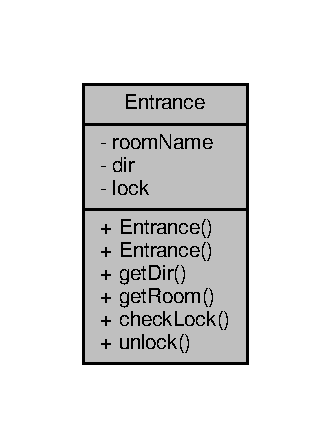
\includegraphics[width=159pt]{class_entrance__coll__graph}
\end{center}
\end{figure}
\subsection*{Public Member Functions}
\begin{DoxyCompactItemize}
\item 
\hyperlink{class_entrance_a88cd27875093371afa47ac0f321716d7}{Entrance} ()
\item 
\hyperlink{class_entrance_a84a2ab9846eb0271b98e22bc131e1ca2}{Entrance} (uwe\+::\+Entrance\+Info ent\+Info)
\item 
std\+::string \hyperlink{class_entrance_a52a2c624cd71effe98fb65b688089dba}{get\+Dir} ()
\item 
std\+::string \hyperlink{class_entrance_abddd96900248aace4478339cfc0b08cb}{get\+Room} ()
\item 
bool \hyperlink{class_entrance_a4bbdb80d7ee6f5fbe3619e9177901d38}{check\+Lock} ()
\item 
void \hyperlink{class_entrance_af14ff07579df1b040890c3a2e447898c}{unlock} ()
\end{DoxyCompactItemize}
\subsection*{Private Attributes}
\begin{DoxyCompactItemize}
\item 
std\+::string \hyperlink{class_entrance_a228a17052cfc8eb772255bee5e9f56ae}{room\+Name}
\item 
std\+::string \hyperlink{class_entrance_ad9ee71c233e33d198c7a6c4d1ec90b46}{dir}
\item 
bool \hyperlink{class_entrance_a16540d02b9f34c068cda79c86dc3df5e}{lock}
\end{DoxyCompactItemize}


\subsection{Constructor \& Destructor Documentation}
\index{Entrance@{Entrance}!Entrance@{Entrance}}
\index{Entrance@{Entrance}!Entrance@{Entrance}}
\subsubsection[{\texorpdfstring{Entrance()}{Entrance()}}]{\setlength{\rightskip}{0pt plus 5cm}Entrance\+::\+Entrance (
\begin{DoxyParamCaption}
{}
\end{DoxyParamCaption}
)}\hypertarget{class_entrance_a88cd27875093371afa47ac0f321716d7}{}\label{class_entrance_a88cd27875093371afa47ac0f321716d7}
\index{Entrance@{Entrance}!Entrance@{Entrance}}
\index{Entrance@{Entrance}!Entrance@{Entrance}}
\subsubsection[{\texorpdfstring{Entrance(uwe\+::\+Entrance\+Info ent\+Info)}{Entrance(uwe::EntranceInfo entInfo)}}]{\setlength{\rightskip}{0pt plus 5cm}Entrance\+::\+Entrance (
\begin{DoxyParamCaption}
\item[{uwe\+::\+Entrance\+Info}]{ent\+Info}
\end{DoxyParamCaption}
)}\hypertarget{class_entrance_a84a2ab9846eb0271b98e22bc131e1ca2}{}\label{class_entrance_a84a2ab9846eb0271b98e22bc131e1ca2}


\subsection{Member Function Documentation}
\index{Entrance@{Entrance}!check\+Lock@{check\+Lock}}
\index{check\+Lock@{check\+Lock}!Entrance@{Entrance}}
\subsubsection[{\texorpdfstring{check\+Lock()}{checkLock()}}]{\setlength{\rightskip}{0pt plus 5cm}bool Entrance\+::check\+Lock (
\begin{DoxyParamCaption}
{}
\end{DoxyParamCaption}
)}\hypertarget{class_entrance_a4bbdb80d7ee6f5fbe3619e9177901d38}{}\label{class_entrance_a4bbdb80d7ee6f5fbe3619e9177901d38}
\index{Entrance@{Entrance}!get\+Dir@{get\+Dir}}
\index{get\+Dir@{get\+Dir}!Entrance@{Entrance}}
\subsubsection[{\texorpdfstring{get\+Dir()}{getDir()}}]{\setlength{\rightskip}{0pt plus 5cm}std\+::string Entrance\+::get\+Dir (
\begin{DoxyParamCaption}
{}
\end{DoxyParamCaption}
)}\hypertarget{class_entrance_a52a2c624cd71effe98fb65b688089dba}{}\label{class_entrance_a52a2c624cd71effe98fb65b688089dba}
\index{Entrance@{Entrance}!get\+Room@{get\+Room}}
\index{get\+Room@{get\+Room}!Entrance@{Entrance}}
\subsubsection[{\texorpdfstring{get\+Room()}{getRoom()}}]{\setlength{\rightskip}{0pt plus 5cm}std\+::string Entrance\+::get\+Room (
\begin{DoxyParamCaption}
{}
\end{DoxyParamCaption}
)}\hypertarget{class_entrance_abddd96900248aace4478339cfc0b08cb}{}\label{class_entrance_abddd96900248aace4478339cfc0b08cb}
\index{Entrance@{Entrance}!unlock@{unlock}}
\index{unlock@{unlock}!Entrance@{Entrance}}
\subsubsection[{\texorpdfstring{unlock()}{unlock()}}]{\setlength{\rightskip}{0pt plus 5cm}void Entrance\+::unlock (
\begin{DoxyParamCaption}
{}
\end{DoxyParamCaption}
)}\hypertarget{class_entrance_af14ff07579df1b040890c3a2e447898c}{}\label{class_entrance_af14ff07579df1b040890c3a2e447898c}


\subsection{Member Data Documentation}
\index{Entrance@{Entrance}!dir@{dir}}
\index{dir@{dir}!Entrance@{Entrance}}
\subsubsection[{\texorpdfstring{dir}{dir}}]{\setlength{\rightskip}{0pt plus 5cm}std\+::string Entrance\+::dir\hspace{0.3cm}{\ttfamily [private]}}\hypertarget{class_entrance_ad9ee71c233e33d198c7a6c4d1ec90b46}{}\label{class_entrance_ad9ee71c233e33d198c7a6c4d1ec90b46}
\index{Entrance@{Entrance}!lock@{lock}}
\index{lock@{lock}!Entrance@{Entrance}}
\subsubsection[{\texorpdfstring{lock}{lock}}]{\setlength{\rightskip}{0pt plus 5cm}bool Entrance\+::lock\hspace{0.3cm}{\ttfamily [private]}}\hypertarget{class_entrance_a16540d02b9f34c068cda79c86dc3df5e}{}\label{class_entrance_a16540d02b9f34c068cda79c86dc3df5e}
\index{Entrance@{Entrance}!room\+Name@{room\+Name}}
\index{room\+Name@{room\+Name}!Entrance@{Entrance}}
\subsubsection[{\texorpdfstring{room\+Name}{roomName}}]{\setlength{\rightskip}{0pt plus 5cm}std\+::string Entrance\+::room\+Name\hspace{0.3cm}{\ttfamily [private]}}\hypertarget{class_entrance_a228a17052cfc8eb772255bee5e9f56ae}{}\label{class_entrance_a228a17052cfc8eb772255bee5e9f56ae}


The documentation for this class was generated from the following files\+:\begin{DoxyCompactItemize}
\item 
include/\hyperlink{entrance_8h}{entrance.\+h}\item 
source/\hyperlink{entrance_8cpp}{entrance.\+cpp}\end{DoxyCompactItemize}

\hypertarget{class_item}{}\section{Item Class Reference}
\label{class_item}\index{Item@{Item}}


{\ttfamily \#include $<$item.\+h$>$}



Collaboration diagram for Item\+:
\nopagebreak
\begin{figure}[H]
\begin{center}
\leavevmode
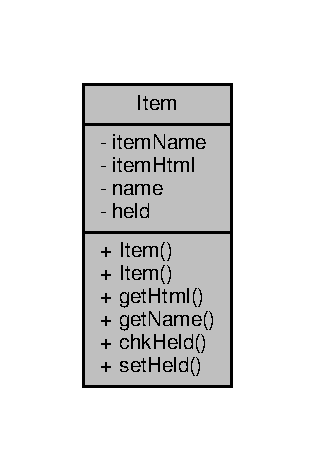
\includegraphics[width=151pt]{class_item__coll__graph}
\end{center}
\end{figure}
\subsection*{Public Member Functions}
\begin{DoxyCompactItemize}
\item 
\hyperlink{class_item_a297720c02984eab37332ae795d22189d}{Item} ()
\item 
\hyperlink{class_item_ab6fbcff91764911e1af1f9a6384b8472}{Item} (std\+::string \hyperlink{class_item_a342b7a351c9ae1c5430aa3ef65b670bd}{name}, std\+::string item\+Desc)
\item 
std\+::string \hyperlink{class_item_a34a7a862e03a25e685bc9d6de8bde908}{get\+Html} ()
\item 
std\+::string \hyperlink{class_item_a4ff297b946505e7956eae16006cada04}{get\+Name} ()
\item 
bool \hyperlink{class_item_ac2ea634d1693b729328307e4a40dbe7a}{chk\+Held} ()
\item 
void \hyperlink{class_item_af3e1688046b6145d02a42eba8443d36d}{set\+Held} ()
\end{DoxyCompactItemize}
\subsection*{Private Attributes}
\begin{DoxyCompactItemize}
\item 
std\+::string \hyperlink{class_item_a17b15dc1e47ddba7e5c98476aeae98a6}{item\+Name}
\item 
std\+::string \hyperlink{class_item_a324a6bcafab4ed84ad92860e061635e9}{item\+Html}
\item 
std\+::string \hyperlink{class_item_a342b7a351c9ae1c5430aa3ef65b670bd}{name}
\item 
bool \hyperlink{class_item_acb32fa26879eb794207306dd7f322f1f}{held}
\end{DoxyCompactItemize}


\subsection{Constructor \& Destructor Documentation}
\index{Item@{Item}!Item@{Item}}
\index{Item@{Item}!Item@{Item}}
\subsubsection[{\texorpdfstring{Item()}{Item()}}]{\setlength{\rightskip}{0pt plus 5cm}Item\+::\+Item (
\begin{DoxyParamCaption}
{}
\end{DoxyParamCaption}
)}\hypertarget{class_item_a297720c02984eab37332ae795d22189d}{}\label{class_item_a297720c02984eab37332ae795d22189d}
\index{Item@{Item}!Item@{Item}}
\index{Item@{Item}!Item@{Item}}
\subsubsection[{\texorpdfstring{Item(std\+::string name, std\+::string item\+Desc)}{Item(std::string name, std::string itemDesc)}}]{\setlength{\rightskip}{0pt plus 5cm}Item\+::\+Item (
\begin{DoxyParamCaption}
\item[{std\+::string}]{name, }
\item[{std\+::string}]{item\+Desc}
\end{DoxyParamCaption}
)}\hypertarget{class_item_ab6fbcff91764911e1af1f9a6384b8472}{}\label{class_item_ab6fbcff91764911e1af1f9a6384b8472}


\subsection{Member Function Documentation}
\index{Item@{Item}!chk\+Held@{chk\+Held}}
\index{chk\+Held@{chk\+Held}!Item@{Item}}
\subsubsection[{\texorpdfstring{chk\+Held()}{chkHeld()}}]{\setlength{\rightskip}{0pt plus 5cm}bool Item\+::chk\+Held (
\begin{DoxyParamCaption}
{}
\end{DoxyParamCaption}
)}\hypertarget{class_item_ac2ea634d1693b729328307e4a40dbe7a}{}\label{class_item_ac2ea634d1693b729328307e4a40dbe7a}
\index{Item@{Item}!get\+Html@{get\+Html}}
\index{get\+Html@{get\+Html}!Item@{Item}}
\subsubsection[{\texorpdfstring{get\+Html()}{getHtml()}}]{\setlength{\rightskip}{0pt plus 5cm}std\+::string Item\+::get\+Html (
\begin{DoxyParamCaption}
{}
\end{DoxyParamCaption}
)}\hypertarget{class_item_a34a7a862e03a25e685bc9d6de8bde908}{}\label{class_item_a34a7a862e03a25e685bc9d6de8bde908}
\index{Item@{Item}!get\+Name@{get\+Name}}
\index{get\+Name@{get\+Name}!Item@{Item}}
\subsubsection[{\texorpdfstring{get\+Name()}{getName()}}]{\setlength{\rightskip}{0pt plus 5cm}std\+::string Item\+::get\+Name (
\begin{DoxyParamCaption}
{}
\end{DoxyParamCaption}
)}\hypertarget{class_item_a4ff297b946505e7956eae16006cada04}{}\label{class_item_a4ff297b946505e7956eae16006cada04}
\index{Item@{Item}!set\+Held@{set\+Held}}
\index{set\+Held@{set\+Held}!Item@{Item}}
\subsubsection[{\texorpdfstring{set\+Held()}{setHeld()}}]{\setlength{\rightskip}{0pt plus 5cm}void Item\+::set\+Held (
\begin{DoxyParamCaption}
{}
\end{DoxyParamCaption}
)}\hypertarget{class_item_af3e1688046b6145d02a42eba8443d36d}{}\label{class_item_af3e1688046b6145d02a42eba8443d36d}


\subsection{Member Data Documentation}
\index{Item@{Item}!held@{held}}
\index{held@{held}!Item@{Item}}
\subsubsection[{\texorpdfstring{held}{held}}]{\setlength{\rightskip}{0pt plus 5cm}bool Item\+::held\hspace{0.3cm}{\ttfamily [private]}}\hypertarget{class_item_acb32fa26879eb794207306dd7f322f1f}{}\label{class_item_acb32fa26879eb794207306dd7f322f1f}
\index{Item@{Item}!item\+Html@{item\+Html}}
\index{item\+Html@{item\+Html}!Item@{Item}}
\subsubsection[{\texorpdfstring{item\+Html}{itemHtml}}]{\setlength{\rightskip}{0pt plus 5cm}std\+::string Item\+::item\+Html\hspace{0.3cm}{\ttfamily [private]}}\hypertarget{class_item_a324a6bcafab4ed84ad92860e061635e9}{}\label{class_item_a324a6bcafab4ed84ad92860e061635e9}
\index{Item@{Item}!item\+Name@{item\+Name}}
\index{item\+Name@{item\+Name}!Item@{Item}}
\subsubsection[{\texorpdfstring{item\+Name}{itemName}}]{\setlength{\rightskip}{0pt plus 5cm}std\+::string Item\+::item\+Name\hspace{0.3cm}{\ttfamily [private]}}\hypertarget{class_item_a17b15dc1e47ddba7e5c98476aeae98a6}{}\label{class_item_a17b15dc1e47ddba7e5c98476aeae98a6}
\index{Item@{Item}!name@{name}}
\index{name@{name}!Item@{Item}}
\subsubsection[{\texorpdfstring{name}{name}}]{\setlength{\rightskip}{0pt plus 5cm}std\+::string Item\+::name\hspace{0.3cm}{\ttfamily [private]}}\hypertarget{class_item_a342b7a351c9ae1c5430aa3ef65b670bd}{}\label{class_item_a342b7a351c9ae1c5430aa3ef65b670bd}


The documentation for this class was generated from the following files\+:\begin{DoxyCompactItemize}
\item 
include/\hyperlink{item_8h}{item.\+h}\item 
source/\hyperlink{item_8cpp}{item.\+cpp}\end{DoxyCompactItemize}

\hypertarget{class_player}{}\section{Player Class Reference}
\label{class_player}\index{Player@{Player}}


{\ttfamily \#include $<$player.\+h$>$}



Collaboration diagram for Player\+:
\nopagebreak
\begin{figure}[H]
\begin{center}
\leavevmode
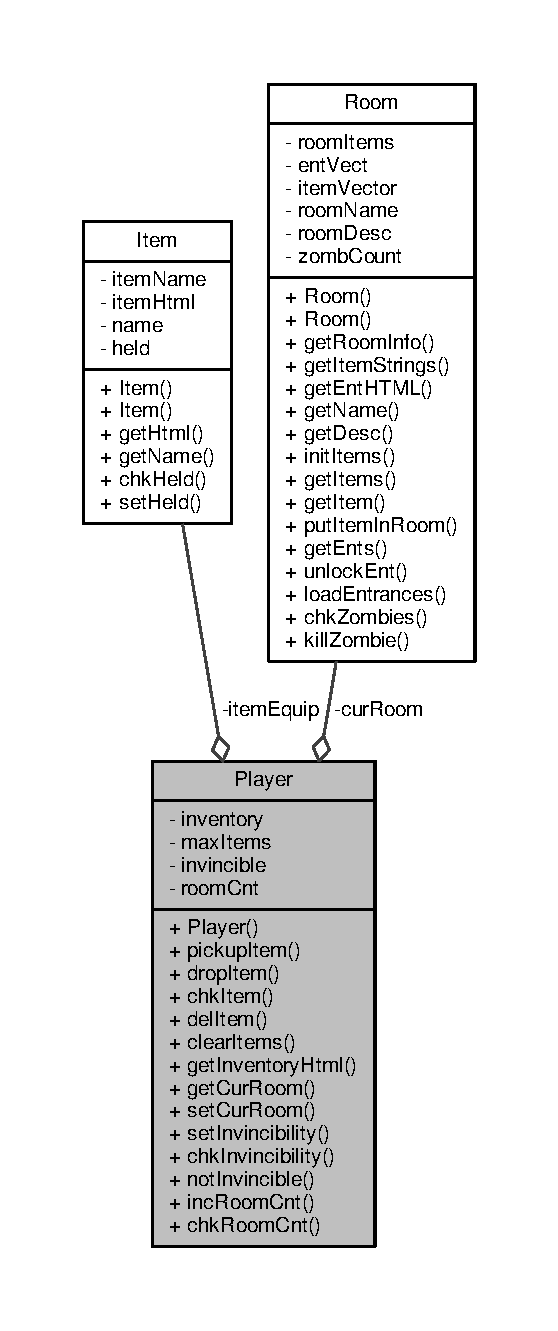
\includegraphics[height=550pt]{class_player__coll__graph}
\end{center}
\end{figure}
\subsection*{Public Member Functions}
\begin{DoxyCompactItemize}
\item 
\hyperlink{class_player_affe0cc3cb714f6deb4e62f0c0d3f1fd8}{Player} ()
\item 
bool \hyperlink{class_player_af2cde98e3e3016f52bcec03c56aec407}{pickup\+Item} (\hyperlink{class_item}{Item} item)
\item 
bool \hyperlink{class_player_adb4031aaf2536a5a7f89e7d194d990e2}{drop\+Item} (std\+::string item)
\item 
bool \hyperlink{class_player_a8c1c3b5c6c5477f32309e93a63b386ff}{chk\+Item} (std\+::string item)
\item 
bool \hyperlink{class_player_a081bbb9e703f1f32eeaa3f9aac6ac327}{del\+Item} (std\+::string item)
\item 
void \hyperlink{class_player_ad6b1c30ffa56aacefb102195a041577d}{clear\+Items} ()
\item 
std\+::string \hyperlink{class_player_ab21f29bdef7ec29545dbb45f2a166ab0}{get\+Inventory\+Html} ()
\item 
\hyperlink{class_room}{Room} $\ast$ \hyperlink{class_player_aa19bb311c830a1e886609eb53502d0b0}{get\+Cur\+Room} ()
\item 
void \hyperlink{class_player_a2e90aee69f3d694edf944d5550fe73f9}{set\+Cur\+Room} (\hyperlink{class_room}{Room} $\ast$room)
\item 
bool \hyperlink{class_player_aebb3bc5a8d6dcbd27acf67ebd4ca6629}{set\+Invincibility} ()
\item 
bool \hyperlink{class_player_aaed2208fc599e76484fde37c38449cb1}{chk\+Invincibility} ()
\item 
bool \hyperlink{class_player_a86a98bb13b3a62ef59742ccb98ad3af5}{not\+Invincible} ()
\item 
void \hyperlink{class_player_a0ddbb83f6ed54aff1818a5f49291f644}{inc\+Room\+Cnt} ()
\item 
int \hyperlink{class_player_a842a4d1798d51aa4e9c4aa31868fe1a6}{chk\+Room\+Cnt} ()
\end{DoxyCompactItemize}
\subsection*{Private Attributes}
\begin{DoxyCompactItemize}
\item 
std\+::vector$<$ \hyperlink{class_item}{Item} $>$ \hyperlink{class_player_ad005856eb5f23892ae9687e601f12f6c}{inventory}
\item 
int \hyperlink{class_player_a903fd9a9a0dd63ddf7e88b901a72fb99}{max\+Items}
\item 
bool \hyperlink{class_player_aaf8419f2a11f79492d1e9081b8913374}{invincible}
\item 
int \hyperlink{class_player_a5de846054e4705449a8b8a2365f2f86c}{room\+Cnt}
\item 
\hyperlink{class_item}{Item} $\ast$ \hyperlink{class_player_ae0c757e73e05e1a7ebf6f2f511db7494}{item\+Equip}
\item 
\hyperlink{class_room}{Room} $\ast$ \hyperlink{class_player_a3be13f6a24a17bd2d199c208a7e96611}{cur\+Room}
\end{DoxyCompactItemize}


\subsection{Constructor \& Destructor Documentation}
\index{Player@{Player}!Player@{Player}}
\index{Player@{Player}!Player@{Player}}
\subsubsection[{\texorpdfstring{Player()}{Player()}}]{\setlength{\rightskip}{0pt plus 5cm}Player\+::\+Player (
\begin{DoxyParamCaption}
{}
\end{DoxyParamCaption}
)}\hypertarget{class_player_affe0cc3cb714f6deb4e62f0c0d3f1fd8}{}\label{class_player_affe0cc3cb714f6deb4e62f0c0d3f1fd8}


\subsection{Member Function Documentation}
\index{Player@{Player}!chk\+Invincibility@{chk\+Invincibility}}
\index{chk\+Invincibility@{chk\+Invincibility}!Player@{Player}}
\subsubsection[{\texorpdfstring{chk\+Invincibility()}{chkInvincibility()}}]{\setlength{\rightskip}{0pt plus 5cm}bool Player\+::chk\+Invincibility (
\begin{DoxyParamCaption}
{}
\end{DoxyParamCaption}
)}\hypertarget{class_player_aaed2208fc599e76484fde37c38449cb1}{}\label{class_player_aaed2208fc599e76484fde37c38449cb1}
\index{Player@{Player}!chk\+Item@{chk\+Item}}
\index{chk\+Item@{chk\+Item}!Player@{Player}}
\subsubsection[{\texorpdfstring{chk\+Item(std\+::string item)}{chkItem(std::string item)}}]{\setlength{\rightskip}{0pt plus 5cm}bool Player\+::chk\+Item (
\begin{DoxyParamCaption}
\item[{std\+::string}]{item}
\end{DoxyParamCaption}
)}\hypertarget{class_player_a8c1c3b5c6c5477f32309e93a63b386ff}{}\label{class_player_a8c1c3b5c6c5477f32309e93a63b386ff}
\index{Player@{Player}!chk\+Room\+Cnt@{chk\+Room\+Cnt}}
\index{chk\+Room\+Cnt@{chk\+Room\+Cnt}!Player@{Player}}
\subsubsection[{\texorpdfstring{chk\+Room\+Cnt()}{chkRoomCnt()}}]{\setlength{\rightskip}{0pt plus 5cm}int Player\+::chk\+Room\+Cnt (
\begin{DoxyParamCaption}
{}
\end{DoxyParamCaption}
)}\hypertarget{class_player_a842a4d1798d51aa4e9c4aa31868fe1a6}{}\label{class_player_a842a4d1798d51aa4e9c4aa31868fe1a6}
\index{Player@{Player}!clear\+Items@{clear\+Items}}
\index{clear\+Items@{clear\+Items}!Player@{Player}}
\subsubsection[{\texorpdfstring{clear\+Items()}{clearItems()}}]{\setlength{\rightskip}{0pt plus 5cm}void Player\+::clear\+Items (
\begin{DoxyParamCaption}
{}
\end{DoxyParamCaption}
)}\hypertarget{class_player_ad6b1c30ffa56aacefb102195a041577d}{}\label{class_player_ad6b1c30ffa56aacefb102195a041577d}
\index{Player@{Player}!del\+Item@{del\+Item}}
\index{del\+Item@{del\+Item}!Player@{Player}}
\subsubsection[{\texorpdfstring{del\+Item(std\+::string item)}{delItem(std::string item)}}]{\setlength{\rightskip}{0pt plus 5cm}bool Player\+::del\+Item (
\begin{DoxyParamCaption}
\item[{std\+::string}]{item}
\end{DoxyParamCaption}
)}\hypertarget{class_player_a081bbb9e703f1f32eeaa3f9aac6ac327}{}\label{class_player_a081bbb9e703f1f32eeaa3f9aac6ac327}
\index{Player@{Player}!drop\+Item@{drop\+Item}}
\index{drop\+Item@{drop\+Item}!Player@{Player}}
\subsubsection[{\texorpdfstring{drop\+Item(std\+::string item)}{dropItem(std::string item)}}]{\setlength{\rightskip}{0pt plus 5cm}bool Player\+::drop\+Item (
\begin{DoxyParamCaption}
\item[{std\+::string}]{item}
\end{DoxyParamCaption}
)}\hypertarget{class_player_adb4031aaf2536a5a7f89e7d194d990e2}{}\label{class_player_adb4031aaf2536a5a7f89e7d194d990e2}
\index{Player@{Player}!get\+Cur\+Room@{get\+Cur\+Room}}
\index{get\+Cur\+Room@{get\+Cur\+Room}!Player@{Player}}
\subsubsection[{\texorpdfstring{get\+Cur\+Room()}{getCurRoom()}}]{\setlength{\rightskip}{0pt plus 5cm}{\bf Room} $\ast$ Player\+::get\+Cur\+Room (
\begin{DoxyParamCaption}
{}
\end{DoxyParamCaption}
)}\hypertarget{class_player_aa19bb311c830a1e886609eb53502d0b0}{}\label{class_player_aa19bb311c830a1e886609eb53502d0b0}
\index{Player@{Player}!get\+Inventory\+Html@{get\+Inventory\+Html}}
\index{get\+Inventory\+Html@{get\+Inventory\+Html}!Player@{Player}}
\subsubsection[{\texorpdfstring{get\+Inventory\+Html()}{getInventoryHtml()}}]{\setlength{\rightskip}{0pt plus 5cm}std\+::string Player\+::get\+Inventory\+Html (
\begin{DoxyParamCaption}
{}
\end{DoxyParamCaption}
)}\hypertarget{class_player_ab21f29bdef7ec29545dbb45f2a166ab0}{}\label{class_player_ab21f29bdef7ec29545dbb45f2a166ab0}
\index{Player@{Player}!inc\+Room\+Cnt@{inc\+Room\+Cnt}}
\index{inc\+Room\+Cnt@{inc\+Room\+Cnt}!Player@{Player}}
\subsubsection[{\texorpdfstring{inc\+Room\+Cnt()}{incRoomCnt()}}]{\setlength{\rightskip}{0pt plus 5cm}void Player\+::inc\+Room\+Cnt (
\begin{DoxyParamCaption}
{}
\end{DoxyParamCaption}
)}\hypertarget{class_player_a0ddbb83f6ed54aff1818a5f49291f644}{}\label{class_player_a0ddbb83f6ed54aff1818a5f49291f644}
\index{Player@{Player}!not\+Invincible@{not\+Invincible}}
\index{not\+Invincible@{not\+Invincible}!Player@{Player}}
\subsubsection[{\texorpdfstring{not\+Invincible()}{notInvincible()}}]{\setlength{\rightskip}{0pt plus 5cm}bool Player\+::not\+Invincible (
\begin{DoxyParamCaption}
{}
\end{DoxyParamCaption}
)}\hypertarget{class_player_a86a98bb13b3a62ef59742ccb98ad3af5}{}\label{class_player_a86a98bb13b3a62ef59742ccb98ad3af5}
\index{Player@{Player}!pickup\+Item@{pickup\+Item}}
\index{pickup\+Item@{pickup\+Item}!Player@{Player}}
\subsubsection[{\texorpdfstring{pickup\+Item(\+Item item)}{pickupItem(Item item)}}]{\setlength{\rightskip}{0pt plus 5cm}bool Player\+::pickup\+Item (
\begin{DoxyParamCaption}
\item[{{\bf Item}}]{item}
\end{DoxyParamCaption}
)}\hypertarget{class_player_af2cde98e3e3016f52bcec03c56aec407}{}\label{class_player_af2cde98e3e3016f52bcec03c56aec407}
\index{Player@{Player}!set\+Cur\+Room@{set\+Cur\+Room}}
\index{set\+Cur\+Room@{set\+Cur\+Room}!Player@{Player}}
\subsubsection[{\texorpdfstring{set\+Cur\+Room(\+Room $\ast$room)}{setCurRoom(Room *room)}}]{\setlength{\rightskip}{0pt plus 5cm}void Player\+::set\+Cur\+Room (
\begin{DoxyParamCaption}
\item[{{\bf Room} $\ast$}]{room}
\end{DoxyParamCaption}
)}\hypertarget{class_player_a2e90aee69f3d694edf944d5550fe73f9}{}\label{class_player_a2e90aee69f3d694edf944d5550fe73f9}
\index{Player@{Player}!set\+Invincibility@{set\+Invincibility}}
\index{set\+Invincibility@{set\+Invincibility}!Player@{Player}}
\subsubsection[{\texorpdfstring{set\+Invincibility()}{setInvincibility()}}]{\setlength{\rightskip}{0pt plus 5cm}bool Player\+::set\+Invincibility (
\begin{DoxyParamCaption}
{}
\end{DoxyParamCaption}
)}\hypertarget{class_player_aebb3bc5a8d6dcbd27acf67ebd4ca6629}{}\label{class_player_aebb3bc5a8d6dcbd27acf67ebd4ca6629}


\subsection{Member Data Documentation}
\index{Player@{Player}!cur\+Room@{cur\+Room}}
\index{cur\+Room@{cur\+Room}!Player@{Player}}
\subsubsection[{\texorpdfstring{cur\+Room}{curRoom}}]{\setlength{\rightskip}{0pt plus 5cm}{\bf Room}$\ast$ Player\+::cur\+Room\hspace{0.3cm}{\ttfamily [private]}}\hypertarget{class_player_a3be13f6a24a17bd2d199c208a7e96611}{}\label{class_player_a3be13f6a24a17bd2d199c208a7e96611}
\index{Player@{Player}!inventory@{inventory}}
\index{inventory@{inventory}!Player@{Player}}
\subsubsection[{\texorpdfstring{inventory}{inventory}}]{\setlength{\rightskip}{0pt plus 5cm}std\+::vector$<${\bf Item}$>$ Player\+::inventory\hspace{0.3cm}{\ttfamily [private]}}\hypertarget{class_player_ad005856eb5f23892ae9687e601f12f6c}{}\label{class_player_ad005856eb5f23892ae9687e601f12f6c}
\index{Player@{Player}!invincible@{invincible}}
\index{invincible@{invincible}!Player@{Player}}
\subsubsection[{\texorpdfstring{invincible}{invincible}}]{\setlength{\rightskip}{0pt plus 5cm}bool Player\+::invincible\hspace{0.3cm}{\ttfamily [private]}}\hypertarget{class_player_aaf8419f2a11f79492d1e9081b8913374}{}\label{class_player_aaf8419f2a11f79492d1e9081b8913374}
\index{Player@{Player}!item\+Equip@{item\+Equip}}
\index{item\+Equip@{item\+Equip}!Player@{Player}}
\subsubsection[{\texorpdfstring{item\+Equip}{itemEquip}}]{\setlength{\rightskip}{0pt plus 5cm}{\bf Item}$\ast$ Player\+::item\+Equip\hspace{0.3cm}{\ttfamily [private]}}\hypertarget{class_player_ae0c757e73e05e1a7ebf6f2f511db7494}{}\label{class_player_ae0c757e73e05e1a7ebf6f2f511db7494}
\index{Player@{Player}!max\+Items@{max\+Items}}
\index{max\+Items@{max\+Items}!Player@{Player}}
\subsubsection[{\texorpdfstring{max\+Items}{maxItems}}]{\setlength{\rightskip}{0pt plus 5cm}int Player\+::max\+Items\hspace{0.3cm}{\ttfamily [private]}}\hypertarget{class_player_a903fd9a9a0dd63ddf7e88b901a72fb99}{}\label{class_player_a903fd9a9a0dd63ddf7e88b901a72fb99}
\index{Player@{Player}!room\+Cnt@{room\+Cnt}}
\index{room\+Cnt@{room\+Cnt}!Player@{Player}}
\subsubsection[{\texorpdfstring{room\+Cnt}{roomCnt}}]{\setlength{\rightskip}{0pt plus 5cm}int Player\+::room\+Cnt\hspace{0.3cm}{\ttfamily [private]}}\hypertarget{class_player_a5de846054e4705449a8b8a2365f2f86c}{}\label{class_player_a5de846054e4705449a8b8a2365f2f86c}


The documentation for this class was generated from the following files\+:\begin{DoxyCompactItemize}
\item 
include/\hyperlink{player_8h}{player.\+h}\item 
source/\hyperlink{player_8cpp}{player.\+cpp}\end{DoxyCompactItemize}

\hypertarget{class_room}{}\section{Room Class Reference}
\label{class_room}\index{Room@{Room}}


{\ttfamily \#include $<$room.\+h$>$}



Collaboration diagram for Room\+:
\nopagebreak
\begin{figure}[H]
\begin{center}
\leavevmode
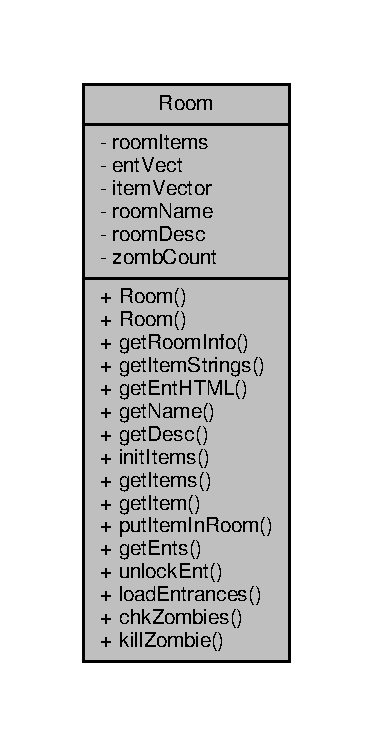
\includegraphics[width=179pt]{class_room__coll__graph}
\end{center}
\end{figure}
\subsection*{Public Member Functions}
\begin{DoxyCompactItemize}
\item 
\hyperlink{class_room_ac6ef93a7d9c3e1d624e025058d5f16ff}{Room} ()
\item 
\hyperlink{class_room_a96f197f3053dfaa506cde4b80978d4bf}{Room} (uwe\+::\+Room\+Info ri, std\+::vector$<$ \hyperlink{class_item}{Item} $>$\hyperlink{class_room_a21e907fa249c8248845a4e001c7b572a}{item\+Vector})
\item 
std\+::string \hyperlink{class_room_a51db5005d72bcaabd2f13b52eb740e30}{get\+Room\+Info} ()
\item 
std\+::string \hyperlink{class_room_a59f42b1d74464cd62fb9691ed2be0c85}{get\+Item\+Strings} ()
\item 
std\+::string \hyperlink{class_room_a75271a20c610a24bfa275953c45dae61}{get\+Ent\+H\+T\+ML} ()
\item 
std\+::string \hyperlink{class_room_ae6a3be5861b657a2cbbada8e67ab7fde}{get\+Name} ()
\item 
std\+::string \hyperlink{class_room_a49b28c0297cd75f6bb94b861dafbb0bd}{get\+Desc} ()
\item 
void \hyperlink{class_room_a7a2ed3178aed3660121882858f269a10}{init\+Items} (std\+::vector$<$ \hyperlink{class_item}{Item} $>$world\+Items)
\item 
std\+::vector$<$ \hyperlink{class_item}{Item} $>$ \hyperlink{class_room_aff3135c3732758a8e176fe5161a193f2}{get\+Items} ()
\item 
bool \hyperlink{class_room_ab838a8ed7f67e2b438a7d96ffbbe6961}{get\+Item} (std\+::string i\+Name, \hyperlink{class_item}{Item} $\ast$ret\+Item)
\item 
void \hyperlink{class_room_a0aefeb033bb51709bc72fe47574568ca}{put\+Item\+In\+Room} (\hyperlink{class_item}{Item} item)
\item 
std\+::vector$<$ \hyperlink{class_entrance}{Entrance} $>$ \hyperlink{class_room_ac4233ee265acfda90b9f159219553e36}{get\+Ents} ()
\item 
void \hyperlink{class_room_a1328ddc5bd5957738335f7c05f21959f}{unlock\+Ent} (std\+::string ent\+Name)
\item 
void \hyperlink{class_room_ae6c0cdda79ffe2c9ce43b816f137a99d}{load\+Entrances} (std\+::vector$<$ uwe\+::\+Entrance\+Info $>$entrances\+J\+S\+ON)
\item 
int \hyperlink{class_room_a9995dfb547b839c817a3f1b107ae3591}{chk\+Zombies} ()
\item 
void \hyperlink{class_room_aaeaf156da5e9ae2980438d495dbb5420}{kill\+Zombie} ()
\end{DoxyCompactItemize}
\subsection*{Private Attributes}
\begin{DoxyCompactItemize}
\item 
std\+::vector$<$ std\+::string $>$ \hyperlink{class_room_af7b9b2ab1bd1eda19d6b893c984d73d7}{room\+Items}
\item 
std\+::vector$<$ \hyperlink{class_entrance}{Entrance} $>$ \hyperlink{class_room_a7e93af067cbea670fd4a4e8addffd09a}{ent\+Vect}
\item 
std\+::vector$<$ \hyperlink{class_item}{Item} $>$ \hyperlink{class_room_a21e907fa249c8248845a4e001c7b572a}{item\+Vector}
\item 
std\+::string \hyperlink{class_room_add2825ea48f72ca1b06ae26c28297cdc}{room\+Name}
\item 
std\+::string \hyperlink{class_room_ae18039ced2c32837f5064961bb33e4e9}{room\+Desc}
\item 
int \hyperlink{class_room_afcddb9fd9012f7838876a64c834a0349}{zomb\+Count}
\end{DoxyCompactItemize}


\subsection{Constructor \& Destructor Documentation}
\index{Room@{Room}!Room@{Room}}
\index{Room@{Room}!Room@{Room}}
\subsubsection[{\texorpdfstring{Room()}{Room()}}]{\setlength{\rightskip}{0pt plus 5cm}Room\+::\+Room (
\begin{DoxyParamCaption}
{}
\end{DoxyParamCaption}
)}\hypertarget{class_room_ac6ef93a7d9c3e1d624e025058d5f16ff}{}\label{class_room_ac6ef93a7d9c3e1d624e025058d5f16ff}
\index{Room@{Room}!Room@{Room}}
\index{Room@{Room}!Room@{Room}}
\subsubsection[{\texorpdfstring{Room(uwe\+::\+Room\+Info ri, std\+::vector$<$ Item $>$item\+Vector)}{Room(uwe::RoomInfo ri, std::vector< Item >itemVector)}}]{\setlength{\rightskip}{0pt plus 5cm}Room\+::\+Room (
\begin{DoxyParamCaption}
\item[{uwe\+::\+Room\+Info}]{ri, }
\item[{std\+::vector$<$ {\bf Item} $>$}]{item\+Vector}
\end{DoxyParamCaption}
)}\hypertarget{class_room_a96f197f3053dfaa506cde4b80978d4bf}{}\label{class_room_a96f197f3053dfaa506cde4b80978d4bf}


\subsection{Member Function Documentation}
\index{Room@{Room}!chk\+Zombies@{chk\+Zombies}}
\index{chk\+Zombies@{chk\+Zombies}!Room@{Room}}
\subsubsection[{\texorpdfstring{chk\+Zombies()}{chkZombies()}}]{\setlength{\rightskip}{0pt plus 5cm}int Room\+::chk\+Zombies (
\begin{DoxyParamCaption}
{}
\end{DoxyParamCaption}
)}\hypertarget{class_room_a9995dfb547b839c817a3f1b107ae3591}{}\label{class_room_a9995dfb547b839c817a3f1b107ae3591}
\index{Room@{Room}!get\+Desc@{get\+Desc}}
\index{get\+Desc@{get\+Desc}!Room@{Room}}
\subsubsection[{\texorpdfstring{get\+Desc()}{getDesc()}}]{\setlength{\rightskip}{0pt plus 5cm}std\+::string Room\+::get\+Desc (
\begin{DoxyParamCaption}
{}
\end{DoxyParamCaption}
)}\hypertarget{class_room_a49b28c0297cd75f6bb94b861dafbb0bd}{}\label{class_room_a49b28c0297cd75f6bb94b861dafbb0bd}
\index{Room@{Room}!get\+Ent\+H\+T\+ML@{get\+Ent\+H\+T\+ML}}
\index{get\+Ent\+H\+T\+ML@{get\+Ent\+H\+T\+ML}!Room@{Room}}
\subsubsection[{\texorpdfstring{get\+Ent\+H\+T\+M\+L()}{getEntHTML()}}]{\setlength{\rightskip}{0pt plus 5cm}std\+::string Room\+::get\+Ent\+H\+T\+ML (
\begin{DoxyParamCaption}
{}
\end{DoxyParamCaption}
)}\hypertarget{class_room_a75271a20c610a24bfa275953c45dae61}{}\label{class_room_a75271a20c610a24bfa275953c45dae61}
\index{Room@{Room}!get\+Ents@{get\+Ents}}
\index{get\+Ents@{get\+Ents}!Room@{Room}}
\subsubsection[{\texorpdfstring{get\+Ents()}{getEnts()}}]{\setlength{\rightskip}{0pt plus 5cm}std\+::vector$<$ {\bf Entrance} $>$ Room\+::get\+Ents (
\begin{DoxyParamCaption}
{}
\end{DoxyParamCaption}
)}\hypertarget{class_room_ac4233ee265acfda90b9f159219553e36}{}\label{class_room_ac4233ee265acfda90b9f159219553e36}
\index{Room@{Room}!get\+Item@{get\+Item}}
\index{get\+Item@{get\+Item}!Room@{Room}}
\subsubsection[{\texorpdfstring{get\+Item(std\+::string i\+Name, Item $\ast$ret\+Item)}{getItem(std::string iName, Item *retItem)}}]{\setlength{\rightskip}{0pt plus 5cm}bool Room\+::get\+Item (
\begin{DoxyParamCaption}
\item[{std\+::string}]{i\+Name, }
\item[{{\bf Item} $\ast$}]{ret\+Item}
\end{DoxyParamCaption}
)}\hypertarget{class_room_ab838a8ed7f67e2b438a7d96ffbbe6961}{}\label{class_room_ab838a8ed7f67e2b438a7d96ffbbe6961}
\index{Room@{Room}!get\+Items@{get\+Items}}
\index{get\+Items@{get\+Items}!Room@{Room}}
\subsubsection[{\texorpdfstring{get\+Items()}{getItems()}}]{\setlength{\rightskip}{0pt plus 5cm}std\+::vector$<$ {\bf Item} $>$ Room\+::get\+Items (
\begin{DoxyParamCaption}
{}
\end{DoxyParamCaption}
)}\hypertarget{class_room_aff3135c3732758a8e176fe5161a193f2}{}\label{class_room_aff3135c3732758a8e176fe5161a193f2}
\index{Room@{Room}!get\+Item\+Strings@{get\+Item\+Strings}}
\index{get\+Item\+Strings@{get\+Item\+Strings}!Room@{Room}}
\subsubsection[{\texorpdfstring{get\+Item\+Strings()}{getItemStrings()}}]{\setlength{\rightskip}{0pt plus 5cm}std\+::string Room\+::get\+Item\+Strings (
\begin{DoxyParamCaption}
{}
\end{DoxyParamCaption}
)}\hypertarget{class_room_a59f42b1d74464cd62fb9691ed2be0c85}{}\label{class_room_a59f42b1d74464cd62fb9691ed2be0c85}
\index{Room@{Room}!get\+Name@{get\+Name}}
\index{get\+Name@{get\+Name}!Room@{Room}}
\subsubsection[{\texorpdfstring{get\+Name()}{getName()}}]{\setlength{\rightskip}{0pt plus 5cm}std\+::string Room\+::get\+Name (
\begin{DoxyParamCaption}
{}
\end{DoxyParamCaption}
)}\hypertarget{class_room_ae6a3be5861b657a2cbbada8e67ab7fde}{}\label{class_room_ae6a3be5861b657a2cbbada8e67ab7fde}
\index{Room@{Room}!get\+Room\+Info@{get\+Room\+Info}}
\index{get\+Room\+Info@{get\+Room\+Info}!Room@{Room}}
\subsubsection[{\texorpdfstring{get\+Room\+Info()}{getRoomInfo()}}]{\setlength{\rightskip}{0pt plus 5cm}std\+::string Room\+::get\+Room\+Info (
\begin{DoxyParamCaption}
{}
\end{DoxyParamCaption}
)}\hypertarget{class_room_a51db5005d72bcaabd2f13b52eb740e30}{}\label{class_room_a51db5005d72bcaabd2f13b52eb740e30}
\index{Room@{Room}!init\+Items@{init\+Items}}
\index{init\+Items@{init\+Items}!Room@{Room}}
\subsubsection[{\texorpdfstring{init\+Items(std\+::vector$<$ Item $>$world\+Items)}{initItems(std::vector< Item >worldItems)}}]{\setlength{\rightskip}{0pt plus 5cm}void Room\+::init\+Items (
\begin{DoxyParamCaption}
\item[{std\+::vector$<$ {\bf Item} $>$}]{world\+Items}
\end{DoxyParamCaption}
)}\hypertarget{class_room_a7a2ed3178aed3660121882858f269a10}{}\label{class_room_a7a2ed3178aed3660121882858f269a10}
\index{Room@{Room}!kill\+Zombie@{kill\+Zombie}}
\index{kill\+Zombie@{kill\+Zombie}!Room@{Room}}
\subsubsection[{\texorpdfstring{kill\+Zombie()}{killZombie()}}]{\setlength{\rightskip}{0pt plus 5cm}void Room\+::kill\+Zombie (
\begin{DoxyParamCaption}
{}
\end{DoxyParamCaption}
)}\hypertarget{class_room_aaeaf156da5e9ae2980438d495dbb5420}{}\label{class_room_aaeaf156da5e9ae2980438d495dbb5420}
\index{Room@{Room}!load\+Entrances@{load\+Entrances}}
\index{load\+Entrances@{load\+Entrances}!Room@{Room}}
\subsubsection[{\texorpdfstring{load\+Entrances(std\+::vector$<$ uwe\+::\+Entrance\+Info $>$entrances\+J\+S\+O\+N)}{loadEntrances(std::vector< uwe::EntranceInfo >entrancesJSON)}}]{\setlength{\rightskip}{0pt plus 5cm}void Room\+::load\+Entrances (
\begin{DoxyParamCaption}
\item[{std\+::vector$<$ uwe\+::\+Entrance\+Info $>$}]{entrances\+J\+S\+ON}
\end{DoxyParamCaption}
)}\hypertarget{class_room_ae6c0cdda79ffe2c9ce43b816f137a99d}{}\label{class_room_ae6c0cdda79ffe2c9ce43b816f137a99d}
\index{Room@{Room}!put\+Item\+In\+Room@{put\+Item\+In\+Room}}
\index{put\+Item\+In\+Room@{put\+Item\+In\+Room}!Room@{Room}}
\subsubsection[{\texorpdfstring{put\+Item\+In\+Room(\+Item item)}{putItemInRoom(Item item)}}]{\setlength{\rightskip}{0pt plus 5cm}void Room\+::put\+Item\+In\+Room (
\begin{DoxyParamCaption}
\item[{{\bf Item}}]{item}
\end{DoxyParamCaption}
)}\hypertarget{class_room_a0aefeb033bb51709bc72fe47574568ca}{}\label{class_room_a0aefeb033bb51709bc72fe47574568ca}
\index{Room@{Room}!unlock\+Ent@{unlock\+Ent}}
\index{unlock\+Ent@{unlock\+Ent}!Room@{Room}}
\subsubsection[{\texorpdfstring{unlock\+Ent(std\+::string ent\+Name)}{unlockEnt(std::string entName)}}]{\setlength{\rightskip}{0pt plus 5cm}void Room\+::unlock\+Ent (
\begin{DoxyParamCaption}
\item[{std\+::string}]{ent\+Name}
\end{DoxyParamCaption}
)}\hypertarget{class_room_a1328ddc5bd5957738335f7c05f21959f}{}\label{class_room_a1328ddc5bd5957738335f7c05f21959f}


\subsection{Member Data Documentation}
\index{Room@{Room}!ent\+Vect@{ent\+Vect}}
\index{ent\+Vect@{ent\+Vect}!Room@{Room}}
\subsubsection[{\texorpdfstring{ent\+Vect}{entVect}}]{\setlength{\rightskip}{0pt plus 5cm}std\+::vector$<${\bf Entrance}$>$ Room\+::ent\+Vect\hspace{0.3cm}{\ttfamily [private]}}\hypertarget{class_room_a7e93af067cbea670fd4a4e8addffd09a}{}\label{class_room_a7e93af067cbea670fd4a4e8addffd09a}
\index{Room@{Room}!item\+Vector@{item\+Vector}}
\index{item\+Vector@{item\+Vector}!Room@{Room}}
\subsubsection[{\texorpdfstring{item\+Vector}{itemVector}}]{\setlength{\rightskip}{0pt plus 5cm}std\+::vector$<${\bf Item}$>$ Room\+::item\+Vector\hspace{0.3cm}{\ttfamily [private]}}\hypertarget{class_room_a21e907fa249c8248845a4e001c7b572a}{}\label{class_room_a21e907fa249c8248845a4e001c7b572a}
\index{Room@{Room}!room\+Desc@{room\+Desc}}
\index{room\+Desc@{room\+Desc}!Room@{Room}}
\subsubsection[{\texorpdfstring{room\+Desc}{roomDesc}}]{\setlength{\rightskip}{0pt plus 5cm}std\+::string Room\+::room\+Desc\hspace{0.3cm}{\ttfamily [private]}}\hypertarget{class_room_ae18039ced2c32837f5064961bb33e4e9}{}\label{class_room_ae18039ced2c32837f5064961bb33e4e9}
\index{Room@{Room}!room\+Items@{room\+Items}}
\index{room\+Items@{room\+Items}!Room@{Room}}
\subsubsection[{\texorpdfstring{room\+Items}{roomItems}}]{\setlength{\rightskip}{0pt plus 5cm}std\+::vector$<$std\+::string$>$ Room\+::room\+Items\hspace{0.3cm}{\ttfamily [private]}}\hypertarget{class_room_af7b9b2ab1bd1eda19d6b893c984d73d7}{}\label{class_room_af7b9b2ab1bd1eda19d6b893c984d73d7}
\index{Room@{Room}!room\+Name@{room\+Name}}
\index{room\+Name@{room\+Name}!Room@{Room}}
\subsubsection[{\texorpdfstring{room\+Name}{roomName}}]{\setlength{\rightskip}{0pt plus 5cm}std\+::string Room\+::room\+Name\hspace{0.3cm}{\ttfamily [private]}}\hypertarget{class_room_add2825ea48f72ca1b06ae26c28297cdc}{}\label{class_room_add2825ea48f72ca1b06ae26c28297cdc}
\index{Room@{Room}!zomb\+Count@{zomb\+Count}}
\index{zomb\+Count@{zomb\+Count}!Room@{Room}}
\subsubsection[{\texorpdfstring{zomb\+Count}{zombCount}}]{\setlength{\rightskip}{0pt plus 5cm}int Room\+::zomb\+Count\hspace{0.3cm}{\ttfamily [private]}}\hypertarget{class_room_afcddb9fd9012f7838876a64c834a0349}{}\label{class_room_afcddb9fd9012f7838876a64c834a0349}


The documentation for this class was generated from the following files\+:\begin{DoxyCompactItemize}
\item 
include/\hyperlink{room_8h}{room.\+h}\item 
source/\hyperlink{room_8cpp}{room.\+cpp}\end{DoxyCompactItemize}

\hypertarget{class_world}{}\section{World Class Reference}
\label{class_world}\index{World@{World}}


{\ttfamily \#include $<$world.\+h$>$}



Collaboration diagram for World\+:
\nopagebreak
\begin{figure}[H]
\begin{center}
\leavevmode
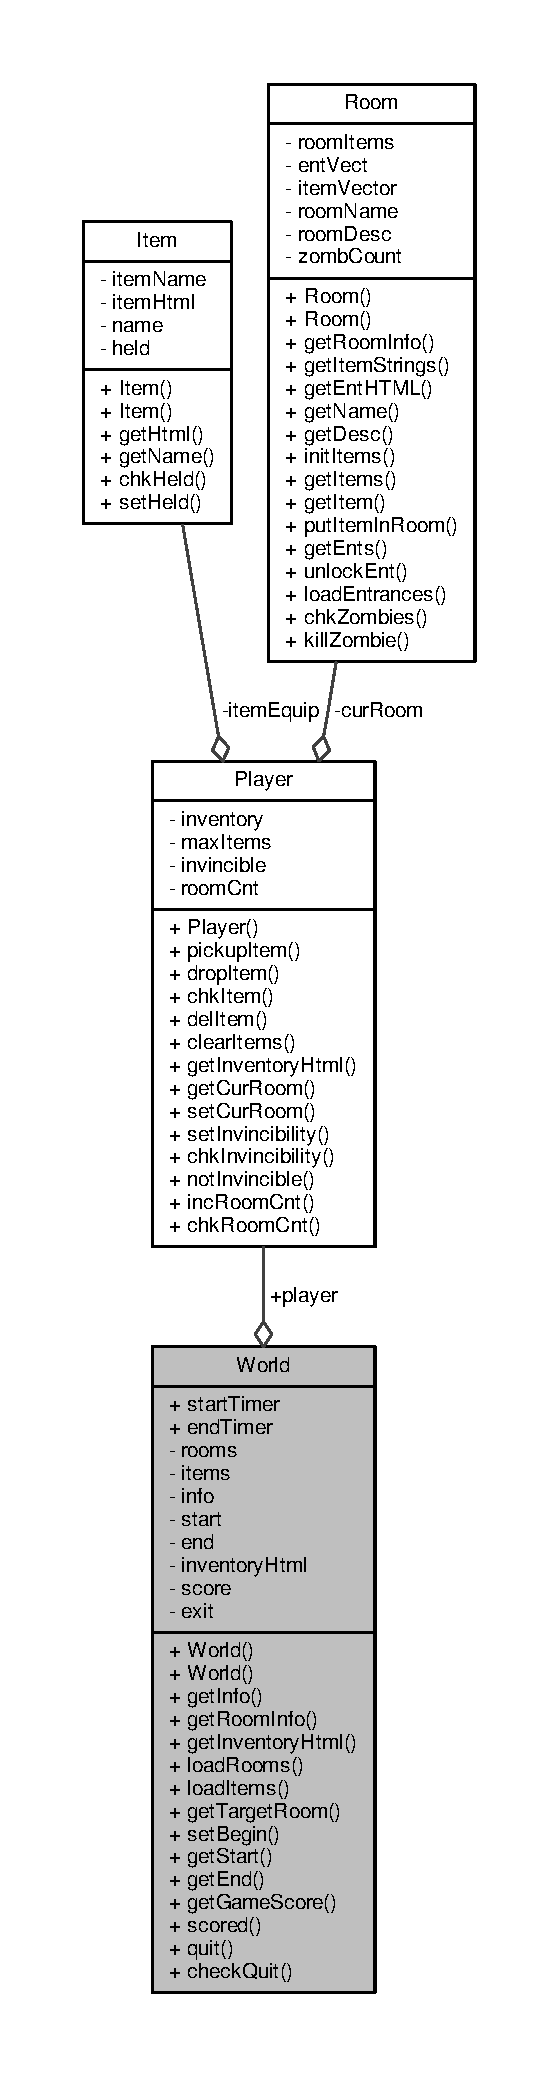
\includegraphics[height=550pt]{class_world__coll__graph}
\end{center}
\end{figure}
\subsection*{Public Member Functions}
\begin{DoxyCompactItemize}
\item 
\hyperlink{class_world_afa39d4e6f714a7a3691ac0c656f5e8a8}{World} ()
\item 
\hyperlink{class_world_aa95deade27bae5842d7faf397e675e30}{World} (uwe\+::\+World\+Loader wl)
\item 
std\+::string \hyperlink{class_world_a35c3f1ee9e59671afd8afe7153080c60}{get\+Info} ()
\item 
std\+::string \hyperlink{class_world_aa45cb41c5134a61443d9e1d8af6638ca}{get\+Room\+Info} ()
\item 
std\+::string \hyperlink{class_world_ae5944d2cac3bb7d2b9ba011b8d159f1d}{get\+Inventory\+Html} ()
\item 
void \hyperlink{class_world_a89353bcb222a0ebc6426916279ac3885}{load\+Rooms} (std\+::vector$<$ uwe\+::\+Room\+Info $>$rooms\+J\+S\+ON)
\item 
void \hyperlink{class_world_a9c7027f0e1a55071bba3193055929f03}{load\+Items} (std\+::vector$<$ uwe\+::\+Item\+Info $>$items\+J\+S\+ON)
\item 
\hyperlink{class_room}{Room} $\ast$ \hyperlink{class_world_a2ec491313aa804a0cc85f240c0a06a39}{get\+Target\+Room} (\hyperlink{class_room}{Room} $\ast$cur\+Room, std\+::string direction, std\+::string $\ast$dir\+Check\+Ret)
\item 
void \hyperlink{class_world_ab8297b76c6b6b91b51b327ee11fe6d5c}{set\+Begin} ()
\item 
\hyperlink{class_room}{Room} $\ast$ \hyperlink{class_world_a84b3872e280eb4f6761a4b1eb0a41e69}{get\+Start} ()
\item 
\hyperlink{class_room}{Room} $\ast$ \hyperlink{class_world_aaea5355cb0778dd10fc079f579c6a60c}{get\+End} ()
\item 
int \hyperlink{class_world_a7eff312b873974bc1fba0fc733e406d7}{get\+Game\+Score} ()
\item 
void \hyperlink{class_world_a59b27842de8fa5982a6deb8333f152d6}{scored} (int amount)
\item 
void \hyperlink{class_world_ac89bad423d24334fa8d9d539a18707ff}{quit} ()
\item 
bool \hyperlink{class_world_a4f052f529eb1af58eeb38d717270b9d7}{check\+Quit} ()
\end{DoxyCompactItemize}
\subsection*{Public Attributes}
\begin{DoxyCompactItemize}
\item 
\hyperlink{class_player}{Player} \hyperlink{class_world_af12585403cef12e595e282dd27948d9a}{player}
\item 
bool \hyperlink{class_world_a7270b9f8836a03add50bffdf20d9d199}{start\+Timer}
\item 
bool \hyperlink{class_world_a16e241b63b668a74380b4db331a4e9ea}{end\+Timer}
\end{DoxyCompactItemize}
\subsection*{Private Attributes}
\begin{DoxyCompactItemize}
\item 
std\+::vector$<$ \hyperlink{class_room}{Room} $>$ \hyperlink{class_world_ab2fda6c8eab2d939323a073c3dd7f1c4}{rooms}
\item 
std\+::vector$<$ \hyperlink{class_item}{Item} $>$ \hyperlink{class_world_a944fe6b2afeecf568d7b904ca4f7c660}{items}
\item 
std\+::string \hyperlink{class_world_a3343e3ea054378472841acb71fc57390}{info}
\item 
std\+::string \hyperlink{class_world_a931da4fdd320f91a2907d3ec740aa071}{start}
\item 
std\+::string \hyperlink{class_world_a5f018ca06c6531c087d2db5dcf33b16f}{end}
\item 
std\+::string \hyperlink{class_world_a7c1c5fac11cd9f7ce463252dc8ead690}{inventory\+Html}
\item 
int \hyperlink{class_world_ae70b4ef5dd9cb9e7336169a25aaee39c}{score}
\item 
bool \hyperlink{class_world_afbd2e53d3a60b74efd0b82e67867d250}{exit}
\end{DoxyCompactItemize}


\subsection{Constructor \& Destructor Documentation}
\index{World@{World}!World@{World}}
\index{World@{World}!World@{World}}
\subsubsection[{\texorpdfstring{World()}{World()}}]{\setlength{\rightskip}{0pt plus 5cm}World\+::\+World (
\begin{DoxyParamCaption}
{}
\end{DoxyParamCaption}
)}\hypertarget{class_world_afa39d4e6f714a7a3691ac0c656f5e8a8}{}\label{class_world_afa39d4e6f714a7a3691ac0c656f5e8a8}
\index{World@{World}!World@{World}}
\index{World@{World}!World@{World}}
\subsubsection[{\texorpdfstring{World(uwe\+::\+World\+Loader wl)}{World(uwe::WorldLoader wl)}}]{\setlength{\rightskip}{0pt plus 5cm}World\+::\+World (
\begin{DoxyParamCaption}
\item[{uwe\+::\+World\+Loader}]{wl}
\end{DoxyParamCaption}
)}\hypertarget{class_world_aa95deade27bae5842d7faf397e675e30}{}\label{class_world_aa95deade27bae5842d7faf397e675e30}


\subsection{Member Function Documentation}
\index{World@{World}!check\+Quit@{check\+Quit}}
\index{check\+Quit@{check\+Quit}!World@{World}}
\subsubsection[{\texorpdfstring{check\+Quit()}{checkQuit()}}]{\setlength{\rightskip}{0pt plus 5cm}bool World\+::check\+Quit (
\begin{DoxyParamCaption}
{}
\end{DoxyParamCaption}
)}\hypertarget{class_world_a4f052f529eb1af58eeb38d717270b9d7}{}\label{class_world_a4f052f529eb1af58eeb38d717270b9d7}
\index{World@{World}!get\+End@{get\+End}}
\index{get\+End@{get\+End}!World@{World}}
\subsubsection[{\texorpdfstring{get\+End()}{getEnd()}}]{\setlength{\rightskip}{0pt plus 5cm}{\bf Room} $\ast$ World\+::get\+End (
\begin{DoxyParamCaption}
{}
\end{DoxyParamCaption}
)}\hypertarget{class_world_aaea5355cb0778dd10fc079f579c6a60c}{}\label{class_world_aaea5355cb0778dd10fc079f579c6a60c}
\index{World@{World}!get\+Game\+Score@{get\+Game\+Score}}
\index{get\+Game\+Score@{get\+Game\+Score}!World@{World}}
\subsubsection[{\texorpdfstring{get\+Game\+Score()}{getGameScore()}}]{\setlength{\rightskip}{0pt plus 5cm}int World\+::get\+Game\+Score (
\begin{DoxyParamCaption}
{}
\end{DoxyParamCaption}
)}\hypertarget{class_world_a7eff312b873974bc1fba0fc733e406d7}{}\label{class_world_a7eff312b873974bc1fba0fc733e406d7}
\index{World@{World}!get\+Info@{get\+Info}}
\index{get\+Info@{get\+Info}!World@{World}}
\subsubsection[{\texorpdfstring{get\+Info()}{getInfo()}}]{\setlength{\rightskip}{0pt plus 5cm}std\+::string World\+::get\+Info (
\begin{DoxyParamCaption}
{}
\end{DoxyParamCaption}
)}\hypertarget{class_world_a35c3f1ee9e59671afd8afe7153080c60}{}\label{class_world_a35c3f1ee9e59671afd8afe7153080c60}
\index{World@{World}!get\+Inventory\+Html@{get\+Inventory\+Html}}
\index{get\+Inventory\+Html@{get\+Inventory\+Html}!World@{World}}
\subsubsection[{\texorpdfstring{get\+Inventory\+Html()}{getInventoryHtml()}}]{\setlength{\rightskip}{0pt plus 5cm}std\+::string World\+::get\+Inventory\+Html (
\begin{DoxyParamCaption}
{}
\end{DoxyParamCaption}
)}\hypertarget{class_world_ae5944d2cac3bb7d2b9ba011b8d159f1d}{}\label{class_world_ae5944d2cac3bb7d2b9ba011b8d159f1d}
\index{World@{World}!get\+Room\+Info@{get\+Room\+Info}}
\index{get\+Room\+Info@{get\+Room\+Info}!World@{World}}
\subsubsection[{\texorpdfstring{get\+Room\+Info()}{getRoomInfo()}}]{\setlength{\rightskip}{0pt plus 5cm}std\+::string World\+::get\+Room\+Info (
\begin{DoxyParamCaption}
{}
\end{DoxyParamCaption}
)}\hypertarget{class_world_aa45cb41c5134a61443d9e1d8af6638ca}{}\label{class_world_aa45cb41c5134a61443d9e1d8af6638ca}
\index{World@{World}!get\+Start@{get\+Start}}
\index{get\+Start@{get\+Start}!World@{World}}
\subsubsection[{\texorpdfstring{get\+Start()}{getStart()}}]{\setlength{\rightskip}{0pt plus 5cm}{\bf Room} $\ast$ World\+::get\+Start (
\begin{DoxyParamCaption}
{}
\end{DoxyParamCaption}
)}\hypertarget{class_world_a84b3872e280eb4f6761a4b1eb0a41e69}{}\label{class_world_a84b3872e280eb4f6761a4b1eb0a41e69}
\index{World@{World}!get\+Target\+Room@{get\+Target\+Room}}
\index{get\+Target\+Room@{get\+Target\+Room}!World@{World}}
\subsubsection[{\texorpdfstring{get\+Target\+Room(\+Room $\ast$cur\+Room, std\+::string direction, std\+::string $\ast$dir\+Check\+Ret)}{getTargetRoom(Room *curRoom, std::string direction, std::string *dirCheckRet)}}]{\setlength{\rightskip}{0pt plus 5cm}{\bf Room} $\ast$ World\+::get\+Target\+Room (
\begin{DoxyParamCaption}
\item[{{\bf Room} $\ast$}]{cur\+Room, }
\item[{std\+::string}]{direction, }
\item[{std\+::string $\ast$}]{dir\+Check\+Ret}
\end{DoxyParamCaption}
)}\hypertarget{class_world_a2ec491313aa804a0cc85f240c0a06a39}{}\label{class_world_a2ec491313aa804a0cc85f240c0a06a39}
\index{World@{World}!load\+Items@{load\+Items}}
\index{load\+Items@{load\+Items}!World@{World}}
\subsubsection[{\texorpdfstring{load\+Items(std\+::vector$<$ uwe\+::\+Item\+Info $>$items\+J\+S\+O\+N)}{loadItems(std::vector< uwe::ItemInfo >itemsJSON)}}]{\setlength{\rightskip}{0pt plus 5cm}void World\+::load\+Items (
\begin{DoxyParamCaption}
\item[{std\+::vector$<$ uwe\+::\+Item\+Info $>$}]{items\+J\+S\+ON}
\end{DoxyParamCaption}
)}\hypertarget{class_world_a9c7027f0e1a55071bba3193055929f03}{}\label{class_world_a9c7027f0e1a55071bba3193055929f03}
\index{World@{World}!load\+Rooms@{load\+Rooms}}
\index{load\+Rooms@{load\+Rooms}!World@{World}}
\subsubsection[{\texorpdfstring{load\+Rooms(std\+::vector$<$ uwe\+::\+Room\+Info $>$rooms\+J\+S\+O\+N)}{loadRooms(std::vector< uwe::RoomInfo >roomsJSON)}}]{\setlength{\rightskip}{0pt plus 5cm}void World\+::load\+Rooms (
\begin{DoxyParamCaption}
\item[{std\+::vector$<$ uwe\+::\+Room\+Info $>$}]{rooms\+J\+S\+ON}
\end{DoxyParamCaption}
)}\hypertarget{class_world_a89353bcb222a0ebc6426916279ac3885}{}\label{class_world_a89353bcb222a0ebc6426916279ac3885}
\index{World@{World}!quit@{quit}}
\index{quit@{quit}!World@{World}}
\subsubsection[{\texorpdfstring{quit()}{quit()}}]{\setlength{\rightskip}{0pt plus 5cm}void World\+::quit (
\begin{DoxyParamCaption}
{}
\end{DoxyParamCaption}
)}\hypertarget{class_world_ac89bad423d24334fa8d9d539a18707ff}{}\label{class_world_ac89bad423d24334fa8d9d539a18707ff}
\index{World@{World}!scored@{scored}}
\index{scored@{scored}!World@{World}}
\subsubsection[{\texorpdfstring{scored(int amount)}{scored(int amount)}}]{\setlength{\rightskip}{0pt plus 5cm}void World\+::scored (
\begin{DoxyParamCaption}
\item[{int}]{amount}
\end{DoxyParamCaption}
)}\hypertarget{class_world_a59b27842de8fa5982a6deb8333f152d6}{}\label{class_world_a59b27842de8fa5982a6deb8333f152d6}
\index{World@{World}!set\+Begin@{set\+Begin}}
\index{set\+Begin@{set\+Begin}!World@{World}}
\subsubsection[{\texorpdfstring{set\+Begin()}{setBegin()}}]{\setlength{\rightskip}{0pt plus 5cm}void World\+::set\+Begin (
\begin{DoxyParamCaption}
{}
\end{DoxyParamCaption}
)}\hypertarget{class_world_ab8297b76c6b6b91b51b327ee11fe6d5c}{}\label{class_world_ab8297b76c6b6b91b51b327ee11fe6d5c}


\subsection{Member Data Documentation}
\index{World@{World}!end@{end}}
\index{end@{end}!World@{World}}
\subsubsection[{\texorpdfstring{end}{end}}]{\setlength{\rightskip}{0pt plus 5cm}std\+::string World\+::end\hspace{0.3cm}{\ttfamily [private]}}\hypertarget{class_world_a5f018ca06c6531c087d2db5dcf33b16f}{}\label{class_world_a5f018ca06c6531c087d2db5dcf33b16f}
\index{World@{World}!end\+Timer@{end\+Timer}}
\index{end\+Timer@{end\+Timer}!World@{World}}
\subsubsection[{\texorpdfstring{end\+Timer}{endTimer}}]{\setlength{\rightskip}{0pt plus 5cm}bool World\+::end\+Timer}\hypertarget{class_world_a16e241b63b668a74380b4db331a4e9ea}{}\label{class_world_a16e241b63b668a74380b4db331a4e9ea}
\index{World@{World}!exit@{exit}}
\index{exit@{exit}!World@{World}}
\subsubsection[{\texorpdfstring{exit}{exit}}]{\setlength{\rightskip}{0pt plus 5cm}bool World\+::exit\hspace{0.3cm}{\ttfamily [private]}}\hypertarget{class_world_afbd2e53d3a60b74efd0b82e67867d250}{}\label{class_world_afbd2e53d3a60b74efd0b82e67867d250}
\index{World@{World}!info@{info}}
\index{info@{info}!World@{World}}
\subsubsection[{\texorpdfstring{info}{info}}]{\setlength{\rightskip}{0pt plus 5cm}std\+::string World\+::info\hspace{0.3cm}{\ttfamily [private]}}\hypertarget{class_world_a3343e3ea054378472841acb71fc57390}{}\label{class_world_a3343e3ea054378472841acb71fc57390}
\index{World@{World}!inventory\+Html@{inventory\+Html}}
\index{inventory\+Html@{inventory\+Html}!World@{World}}
\subsubsection[{\texorpdfstring{inventory\+Html}{inventoryHtml}}]{\setlength{\rightskip}{0pt plus 5cm}std\+::string World\+::inventory\+Html\hspace{0.3cm}{\ttfamily [private]}}\hypertarget{class_world_a7c1c5fac11cd9f7ce463252dc8ead690}{}\label{class_world_a7c1c5fac11cd9f7ce463252dc8ead690}
\index{World@{World}!items@{items}}
\index{items@{items}!World@{World}}
\subsubsection[{\texorpdfstring{items}{items}}]{\setlength{\rightskip}{0pt plus 5cm}std\+::vector$<${\bf Item}$>$ World\+::items\hspace{0.3cm}{\ttfamily [private]}}\hypertarget{class_world_a944fe6b2afeecf568d7b904ca4f7c660}{}\label{class_world_a944fe6b2afeecf568d7b904ca4f7c660}
\index{World@{World}!player@{player}}
\index{player@{player}!World@{World}}
\subsubsection[{\texorpdfstring{player}{player}}]{\setlength{\rightskip}{0pt plus 5cm}{\bf Player} World\+::player}\hypertarget{class_world_af12585403cef12e595e282dd27948d9a}{}\label{class_world_af12585403cef12e595e282dd27948d9a}
\index{World@{World}!rooms@{rooms}}
\index{rooms@{rooms}!World@{World}}
\subsubsection[{\texorpdfstring{rooms}{rooms}}]{\setlength{\rightskip}{0pt plus 5cm}std\+::vector$<${\bf Room}$>$ World\+::rooms\hspace{0.3cm}{\ttfamily [private]}}\hypertarget{class_world_ab2fda6c8eab2d939323a073c3dd7f1c4}{}\label{class_world_ab2fda6c8eab2d939323a073c3dd7f1c4}
\index{World@{World}!score@{score}}
\index{score@{score}!World@{World}}
\subsubsection[{\texorpdfstring{score}{score}}]{\setlength{\rightskip}{0pt plus 5cm}int World\+::score\hspace{0.3cm}{\ttfamily [private]}}\hypertarget{class_world_ae70b4ef5dd9cb9e7336169a25aaee39c}{}\label{class_world_ae70b4ef5dd9cb9e7336169a25aaee39c}
\index{World@{World}!start@{start}}
\index{start@{start}!World@{World}}
\subsubsection[{\texorpdfstring{start}{start}}]{\setlength{\rightskip}{0pt plus 5cm}std\+::string World\+::start\hspace{0.3cm}{\ttfamily [private]}}\hypertarget{class_world_a931da4fdd320f91a2907d3ec740aa071}{}\label{class_world_a931da4fdd320f91a2907d3ec740aa071}
\index{World@{World}!start\+Timer@{start\+Timer}}
\index{start\+Timer@{start\+Timer}!World@{World}}
\subsubsection[{\texorpdfstring{start\+Timer}{startTimer}}]{\setlength{\rightskip}{0pt plus 5cm}bool World\+::start\+Timer}\hypertarget{class_world_a7270b9f8836a03add50bffdf20d9d199}{}\label{class_world_a7270b9f8836a03add50bffdf20d9d199}


The documentation for this class was generated from the following files\+:\begin{DoxyCompactItemize}
\item 
include/\hyperlink{world_8h}{world.\+h}\item 
source/\hyperlink{world_8cpp}{world.\+cpp}\end{DoxyCompactItemize}

\hypertarget{class_zombie_bot}{}\section{Zombie\+Bot Class Reference}
\label{class_zombie_bot}\index{Zombie\+Bot@{Zombie\+Bot}}


{\ttfamily \#include $<$Zombie\+Bot.\+h$>$}



Inheritance diagram for Zombie\+Bot\+:
\nopagebreak
\begin{figure}[H]
\begin{center}
\leavevmode
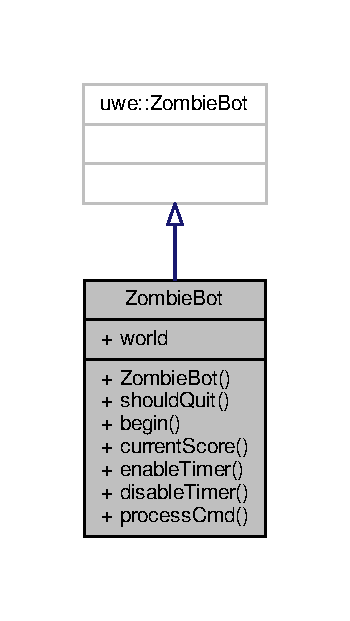
\includegraphics[width=168pt]{class_zombie_bot__inherit__graph}
\end{center}
\end{figure}


Collaboration diagram for Zombie\+Bot\+:
\nopagebreak
\begin{figure}[H]
\begin{center}
\leavevmode
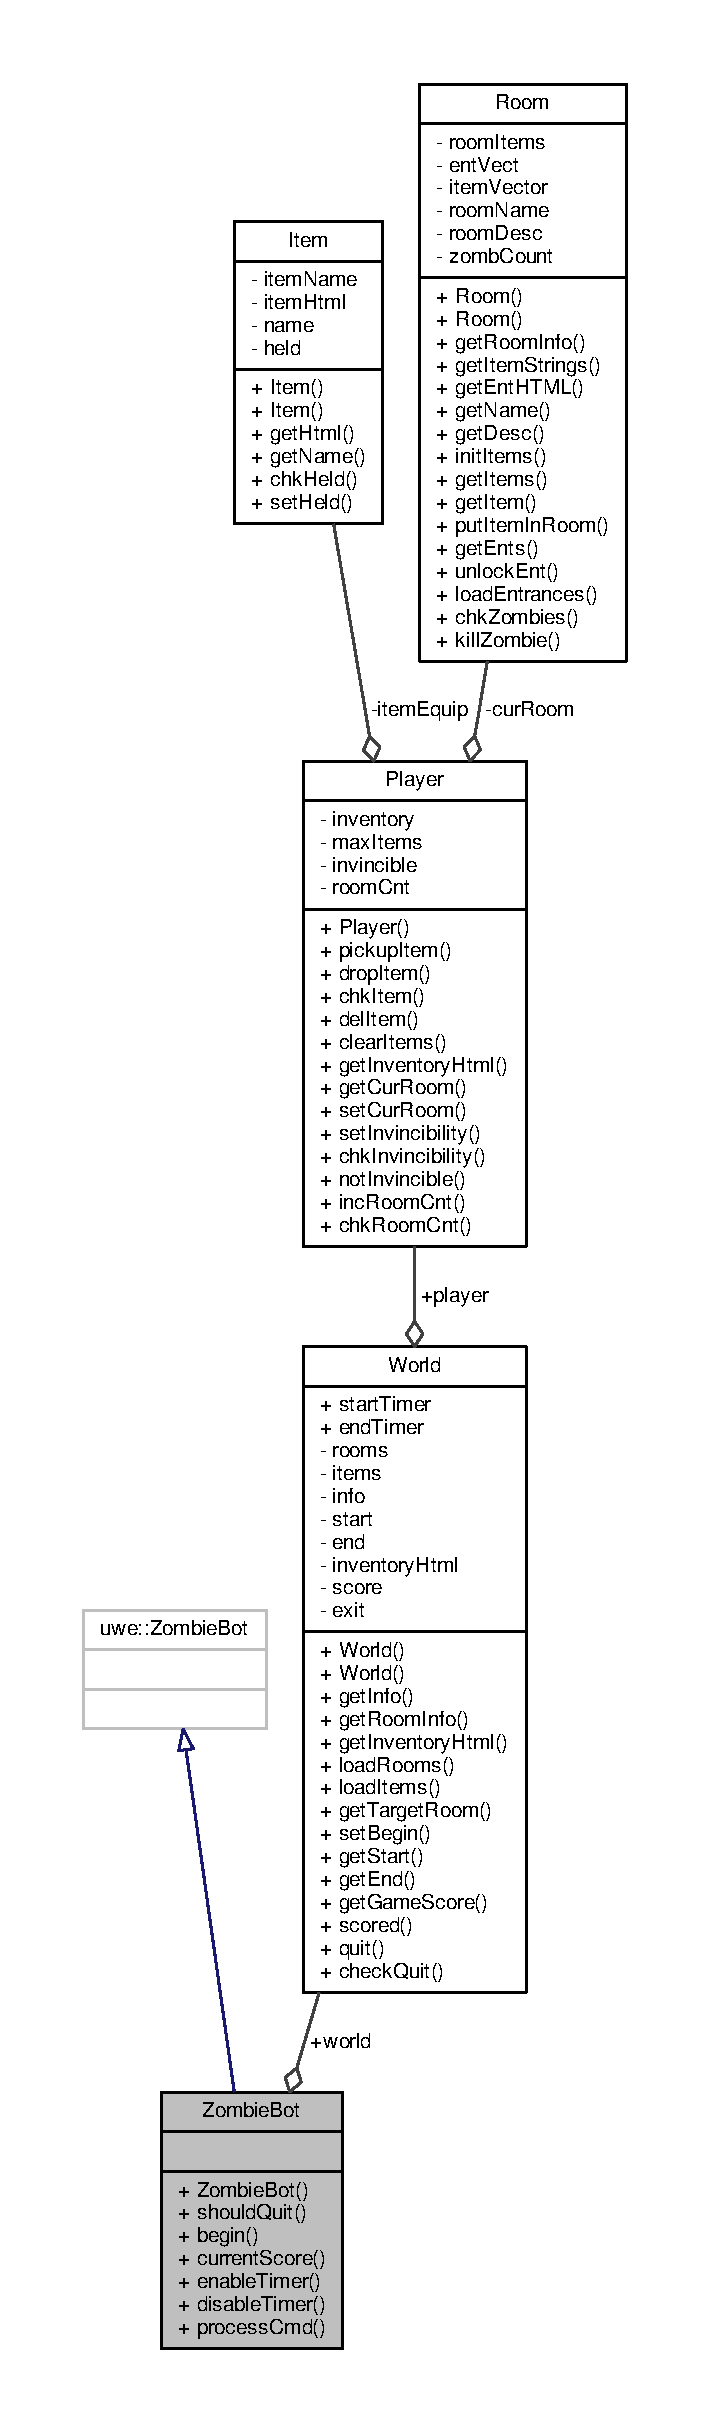
\includegraphics[height=550pt]{class_zombie_bot__coll__graph}
\end{center}
\end{figure}
\subsection*{Public Member Functions}
\begin{DoxyCompactItemize}
\item 
\hyperlink{class_zombie_bot_a1876a669a2bca3d893bd5685b96a8fc7}{Zombie\+Bot} (\hyperlink{class_world}{World} w)
\item 
bool \hyperlink{class_zombie_bot_ae0d559ee494734cb30f29966ce548fae}{should\+Quit} () override
\item 
std\+::string \hyperlink{class_zombie_bot_ab0ad3b297aaa0614eaf335a254044c6f}{begin} () override
\item 
int \hyperlink{class_zombie_bot_a4a470bb8e1bf9f9cafa5846bbae10efd}{current\+Score} () override
\item 
bool \hyperlink{class_zombie_bot_af93d1514656fcf73c9a705fc220c6e5e}{enable\+Timer} () override
\item 
bool \hyperlink{class_zombie_bot_a6078092634dea0a6db55f0377ed3eaa9}{disable\+Timer} () override
\item 
std\+::vector$<$ std\+::string $>$ \hyperlink{class_zombie_bot_a7bdd6cb1af9514dd5afc61066e83d40c}{process\+Cmd} (std\+::string cmd) override
\end{DoxyCompactItemize}
\subsection*{Public Attributes}
\begin{DoxyCompactItemize}
\item 
\hyperlink{class_world}{World} \hyperlink{class_zombie_bot_ae4c9fe36c717e85cc6f0b71ea9c3a4f8}{world}
\end{DoxyCompactItemize}


\subsection{Constructor \& Destructor Documentation}
\index{Zombie\+Bot@{Zombie\+Bot}!Zombie\+Bot@{Zombie\+Bot}}
\index{Zombie\+Bot@{Zombie\+Bot}!Zombie\+Bot@{Zombie\+Bot}}
\subsubsection[{\texorpdfstring{Zombie\+Bot(\+World w)}{ZombieBot(World w)}}]{\setlength{\rightskip}{0pt plus 5cm}Zombie\+Bot\+::\+Zombie\+Bot (
\begin{DoxyParamCaption}
\item[{{\bf World}}]{w}
\end{DoxyParamCaption}
)}\hypertarget{class_zombie_bot_a1876a669a2bca3d893bd5685b96a8fc7}{}\label{class_zombie_bot_a1876a669a2bca3d893bd5685b96a8fc7}


\subsection{Member Function Documentation}
\index{Zombie\+Bot@{Zombie\+Bot}!begin@{begin}}
\index{begin@{begin}!Zombie\+Bot@{Zombie\+Bot}}
\subsubsection[{\texorpdfstring{begin() override}{begin() override}}]{\setlength{\rightskip}{0pt plus 5cm}std\+::string Zombie\+Bot\+::begin (
\begin{DoxyParamCaption}
{}
\end{DoxyParamCaption}
)\hspace{0.3cm}{\ttfamily [override]}}\hypertarget{class_zombie_bot_ab0ad3b297aaa0614eaf335a254044c6f}{}\label{class_zombie_bot_ab0ad3b297aaa0614eaf335a254044c6f}
text to be displayed at beginning of game \begin{DoxyReturn}{Returns}
text to be displayed 
\end{DoxyReturn}
\index{Zombie\+Bot@{Zombie\+Bot}!current\+Score@{current\+Score}}
\index{current\+Score@{current\+Score}!Zombie\+Bot@{Zombie\+Bot}}
\subsubsection[{\texorpdfstring{current\+Score() override}{currentScore() override}}]{\setlength{\rightskip}{0pt plus 5cm}int Zombie\+Bot\+::current\+Score (
\begin{DoxyParamCaption}
{}
\end{DoxyParamCaption}
)\hspace{0.3cm}{\ttfamily [override]}}\hypertarget{class_zombie_bot_a4a470bb8e1bf9f9cafa5846bbae10efd}{}\label{class_zombie_bot_a4a470bb8e1bf9f9cafa5846bbae10efd}
compute current score \begin{DoxyReturn}{Returns}
current score 
\end{DoxyReturn}
\index{Zombie\+Bot@{Zombie\+Bot}!disable\+Timer@{disable\+Timer}}
\index{disable\+Timer@{disable\+Timer}!Zombie\+Bot@{Zombie\+Bot}}
\subsubsection[{\texorpdfstring{disable\+Timer() override}{disableTimer() override}}]{\setlength{\rightskip}{0pt plus 5cm}bool Zombie\+Bot\+::disable\+Timer (
\begin{DoxyParamCaption}
{}
\end{DoxyParamCaption}
)\hspace{0.3cm}{\ttfamily [override]}}\hypertarget{class_zombie_bot_a6078092634dea0a6db55f0377ed3eaa9}{}\label{class_zombie_bot_a6078092634dea0a6db55f0377ed3eaa9}
should zombie timer be disabled \begin{DoxyReturn}{Returns}
true if timer should be disabled, otherwise false 
\end{DoxyReturn}
\index{Zombie\+Bot@{Zombie\+Bot}!enable\+Timer@{enable\+Timer}}
\index{enable\+Timer@{enable\+Timer}!Zombie\+Bot@{Zombie\+Bot}}
\subsubsection[{\texorpdfstring{enable\+Timer() override}{enableTimer() override}}]{\setlength{\rightskip}{0pt plus 5cm}bool Zombie\+Bot\+::enable\+Timer (
\begin{DoxyParamCaption}
{}
\end{DoxyParamCaption}
)\hspace{0.3cm}{\ttfamily [override]}}\hypertarget{class_zombie_bot_af93d1514656fcf73c9a705fc220c6e5e}{}\label{class_zombie_bot_af93d1514656fcf73c9a705fc220c6e5e}
should zombie timer be enabled \begin{DoxyReturn}{Returns}
true if timer should be enabled, otherwise false 
\end{DoxyReturn}
\index{Zombie\+Bot@{Zombie\+Bot}!process\+Cmd@{process\+Cmd}}
\index{process\+Cmd@{process\+Cmd}!Zombie\+Bot@{Zombie\+Bot}}
\subsubsection[{\texorpdfstring{process\+Cmd(std\+::string cmd) override}{processCmd(std::string cmd) override}}]{\setlength{\rightskip}{0pt plus 5cm}std\+::vector$<$ std\+::string $>$ Zombie\+Bot\+::process\+Cmd (
\begin{DoxyParamCaption}
\item[{std\+::string}]{cmd}
\end{DoxyParamCaption}
)\hspace{0.3cm}{\ttfamily [override]}}\hypertarget{class_zombie_bot_a7bdd6cb1af9514dd5afc61066e83d40c}{}\label{class_zombie_bot_a7bdd6cb1af9514dd5afc61066e83d40c}
process player commands.~\newline
~\newline
 The set of commands are as follows\+:~\newline
 
\begin{DoxyItemize}
\item info -\/ return the info string for the world. 
\item look -\/ return the H\+T\+ML representing the view of the current room. this should include entrances, items, and so on.~\newline
  
\item move dir -\/ try and move in the direction dir. if there is an extrance in that direction, then if it is not locked, move through to the connected room, return message about new room. if can\textquotesingle{}t move, because no entrance in that direction, or entrance is locked, then return a message to that effect.~\newline
  
\item one entry to a room if it contains zombies, then the next time the method \hyperlink{class_zombie_bot_af93d1514656fcf73c9a705fc220c6e5e}{enable\+Timer()} is called it should return true, just the one time. This will cause the client to start the Zombie kill timer event, displaying a Zombie and timer, to show the player that they will die if the zombie(s) is not killed in time.~\newline
  
\item pickup item -\/ pick up item from room, if item exits then this should cause it to be removed from room and get added to players inventory, and return message to say picked up. if it does not exist, then return message to that effect.~\newline
 The users score should be increased by one, each time an item is picked up.  
\item kill -\/ if the room contains at least one zombie and players inventory contains either a Daisy or Chainsaw, then one should be killed (i.\+e. zombie count drops by one), return a message to inform the user that a zombie has died. if kill is succcessful, then the player\textquotesingle{}s inventory should have one less Daisy or Chainsaw.~\newline
 if no zombies, then nothing happens.  
\item if the zombie timer was running, i.\+e. a call to \hyperlink{class_zombie_bot_af93d1514656fcf73c9a705fc220c6e5e}{enable\+Timer()} had returned true for the current room, then if the zombie count is now zero, then \hyperlink{class_zombie_bot_a6078092634dea0a6db55f0377ed3eaa9}{disable\+Timer()} should return true, one time, to tell the client to stop the zombie timer.~\newline
  
\item drop item -\/ drop an item into room from inventory. if the item is not in inventory, then nothing happens, otherwise it should be removed, when added to room. return a message to say item dropped.~\newline
  
\item timerexpired -\/ the client\textquotesingle{}s zombie timer expired before all zombies in the current room were killed and so the player is dead. \hyperlink{class_zombie_bot_ae0d559ee494734cb30f29966ce548fae}{should\+Quit()} should now return true.  
\item quit -\/ \hyperlink{class_zombie_bot_ae0d559ee494734cb30f29966ce548fae}{should\+Quit()} should now return true.  
\item inventory -\/ return H\+T\+ML to display the players current inventory.  
\item anything else -\/ return H\+T\+ML saying \char`\"{}\+That\textquotesingle{}s not a verb I recognise.\char`\"{}  
\end{DoxyItemize}
\begin{DoxyParams}{Parameters}
{\em cmd} & to be processed \\
\hline
\end{DoxyParams}
\begin{DoxyReturn}{Returns}
output to be displayed. each element in the list returned is in H\+T\+ML and will be output in the clients display window 
\end{DoxyReturn}
\index{Zombie\+Bot@{Zombie\+Bot}!should\+Quit@{should\+Quit}}
\index{should\+Quit@{should\+Quit}!Zombie\+Bot@{Zombie\+Bot}}
\subsubsection[{\texorpdfstring{should\+Quit() override}{shouldQuit() override}}]{\setlength{\rightskip}{0pt plus 5cm}bool Zombie\+Bot\+::should\+Quit (
\begin{DoxyParamCaption}
{}
\end{DoxyParamCaption}
)\hspace{0.3cm}{\ttfamily [override]}}\hypertarget{class_zombie_bot_ae0d559ee494734cb30f29966ce548fae}{}\label{class_zombie_bot_ae0d559ee494734cb30f29966ce548fae}
should game quit \begin{DoxyReturn}{Returns}
return true if exit program, otherwise false 
\end{DoxyReturn}


\subsection{Member Data Documentation}
\index{Zombie\+Bot@{Zombie\+Bot}!world@{world}}
\index{world@{world}!Zombie\+Bot@{Zombie\+Bot}}
\subsubsection[{\texorpdfstring{world}{world}}]{\setlength{\rightskip}{0pt plus 5cm}{\bf World} Zombie\+Bot\+::world}\hypertarget{class_zombie_bot_ae4c9fe36c717e85cc6f0b71ea9c3a4f8}{}\label{class_zombie_bot_ae4c9fe36c717e85cc6f0b71ea9c3a4f8}


The documentation for this class was generated from the following files\+:\begin{DoxyCompactItemize}
\item 
include/\hyperlink{_zombie_bot_8h}{Zombie\+Bot.\+h}\item 
source/\hyperlink{_zombie_bot_8cpp}{Zombie\+Bot.\+cpp}\end{DoxyCompactItemize}

\chapter{File Documentation}
\hypertarget{entrance_8h}{}\section{include/entrance.h File Reference}
\label{entrance_8h}\index{include/entrance.\+h@{include/entrance.\+h}}
{\ttfamily \#include $<$zombies/\+World\+Loader.\+h$>$}\\*
{\ttfamily \#include $<$ufcfgl-\/30-\/1.\+h$>$}\\*
Include dependency graph for entrance.\+h\+:
\nopagebreak
\begin{figure}[H]
\begin{center}
\leavevmode
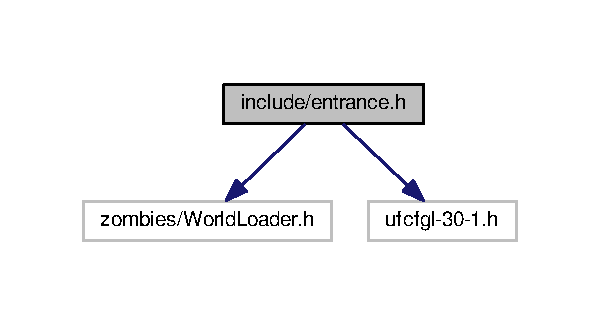
\includegraphics[width=288pt]{entrance_8h__incl}
\end{center}
\end{figure}
This graph shows which files directly or indirectly include this file\+:
\nopagebreak
\begin{figure}[H]
\begin{center}
\leavevmode
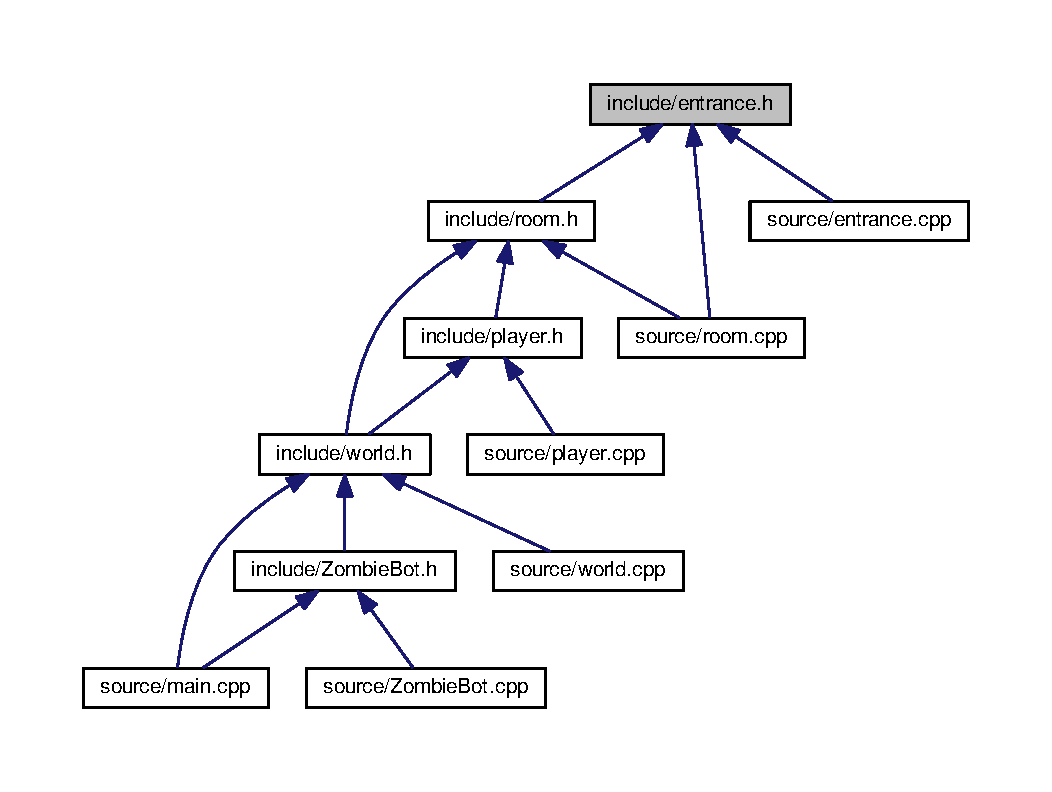
\includegraphics[width=350pt]{entrance_8h__dep__incl}
\end{center}
\end{figure}
\subsection*{Classes}
\begin{DoxyCompactItemize}
\item 
class \hyperlink{class_entrance}{Entrance}
\end{DoxyCompactItemize}

\hypertarget{item_8h}{}\section{include/item.h File Reference}
\label{item_8h}\index{include/item.\+h@{include/item.\+h}}
{\ttfamily \#include $<$ufcfgl-\/30-\/1.\+h$>$}\\*
Include dependency graph for item.\+h\+:
\nopagebreak
\begin{figure}[H]
\begin{center}
\leavevmode
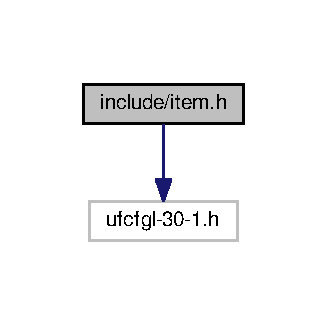
\includegraphics[width=157pt]{item_8h__incl}
\end{center}
\end{figure}
This graph shows which files directly or indirectly include this file\+:
\nopagebreak
\begin{figure}[H]
\begin{center}
\leavevmode
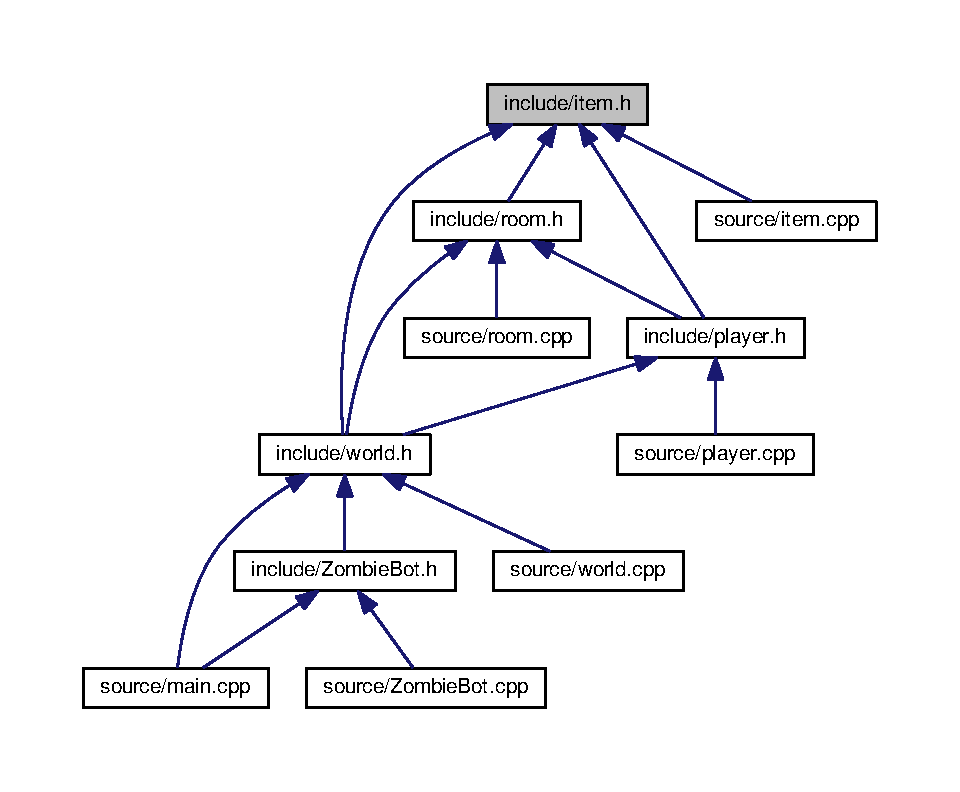
\includegraphics[width=350pt]{item_8h__dep__incl}
\end{center}
\end{figure}
\subsection*{Classes}
\begin{DoxyCompactItemize}
\item 
class \hyperlink{class_item}{Item}
\end{DoxyCompactItemize}

\hypertarget{player_8h}{}\section{include/player.h File Reference}
\label{player_8h}\index{include/player.\+h@{include/player.\+h}}
{\ttfamily \#include \char`\"{}item.\+h\char`\"{}}\\*
{\ttfamily \#include \char`\"{}room.\+h\char`\"{}}\\*
Include dependency graph for player.\+h\+:
\nopagebreak
\begin{figure}[H]
\begin{center}
\leavevmode
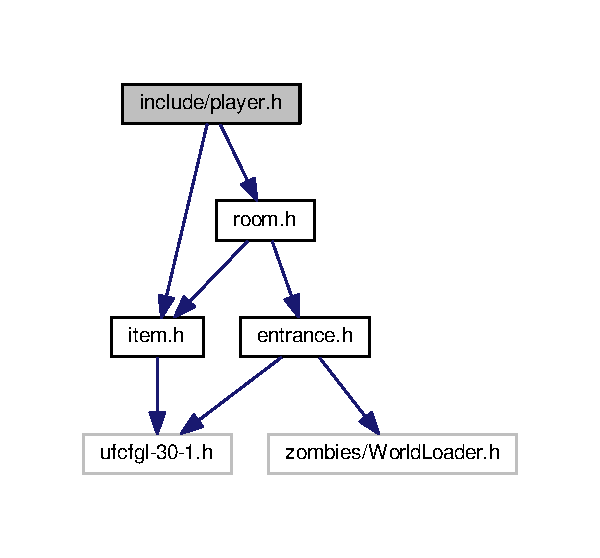
\includegraphics[width=288pt]{player_8h__incl}
\end{center}
\end{figure}
This graph shows which files directly or indirectly include this file\+:
\nopagebreak
\begin{figure}[H]
\begin{center}
\leavevmode
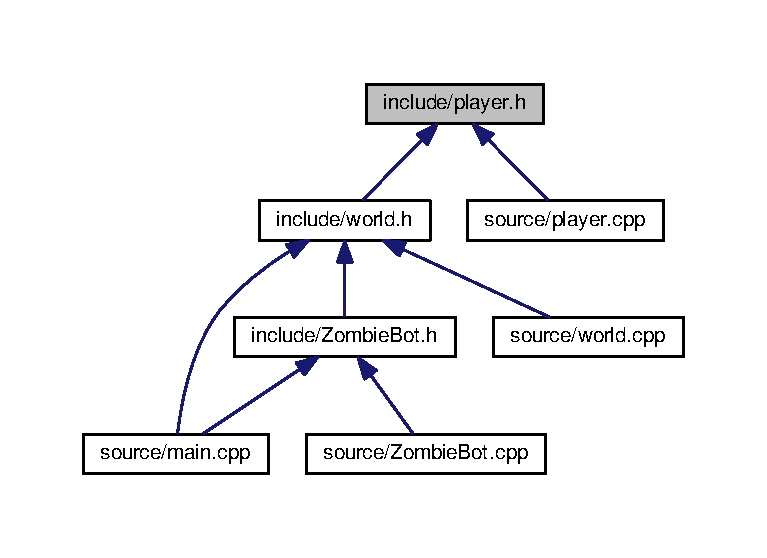
\includegraphics[width=350pt]{player_8h__dep__incl}
\end{center}
\end{figure}
\subsection*{Classes}
\begin{DoxyCompactItemize}
\item 
class \hyperlink{class_player}{Player}
\end{DoxyCompactItemize}

\hypertarget{room_8h}{}\section{include/room.h File Reference}
\label{room_8h}\index{include/room.\+h@{include/room.\+h}}
{\ttfamily \#include \char`\"{}item.\+h\char`\"{}}\\*
{\ttfamily \#include \char`\"{}entrance.\+h\char`\"{}}\\*
Include dependency graph for room.\+h\+:
\nopagebreak
\begin{figure}[H]
\begin{center}
\leavevmode
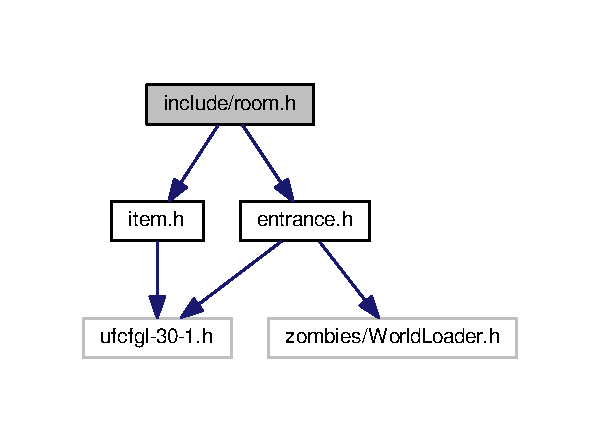
\includegraphics[width=288pt]{room_8h__incl}
\end{center}
\end{figure}
This graph shows which files directly or indirectly include this file\+:
\nopagebreak
\begin{figure}[H]
\begin{center}
\leavevmode
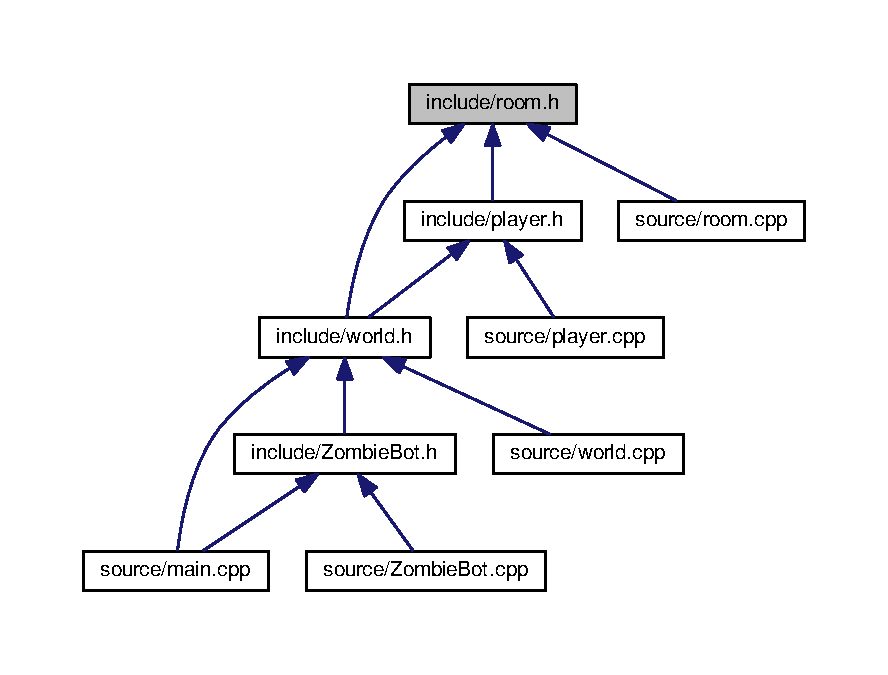
\includegraphics[width=350pt]{room_8h__dep__incl}
\end{center}
\end{figure}
\subsection*{Classes}
\begin{DoxyCompactItemize}
\item 
class \hyperlink{class_room}{Room}
\end{DoxyCompactItemize}

\hypertarget{world_8h}{}\section{include/world.h File Reference}
\label{world_8h}\index{include/world.\+h@{include/world.\+h}}
{\ttfamily \#include $<$ufcfgl-\/30-\/1.\+h$>$}\\*
{\ttfamily \#include $<$zombies/\+World\+Loader.\+h$>$}\\*
{\ttfamily \#include \char`\"{}room.\+h\char`\"{}}\\*
{\ttfamily \#include \char`\"{}item.\+h\char`\"{}}\\*
{\ttfamily \#include \char`\"{}player.\+h\char`\"{}}\\*
Include dependency graph for world.\+h\+:
\nopagebreak
\begin{figure}[H]
\begin{center}
\leavevmode
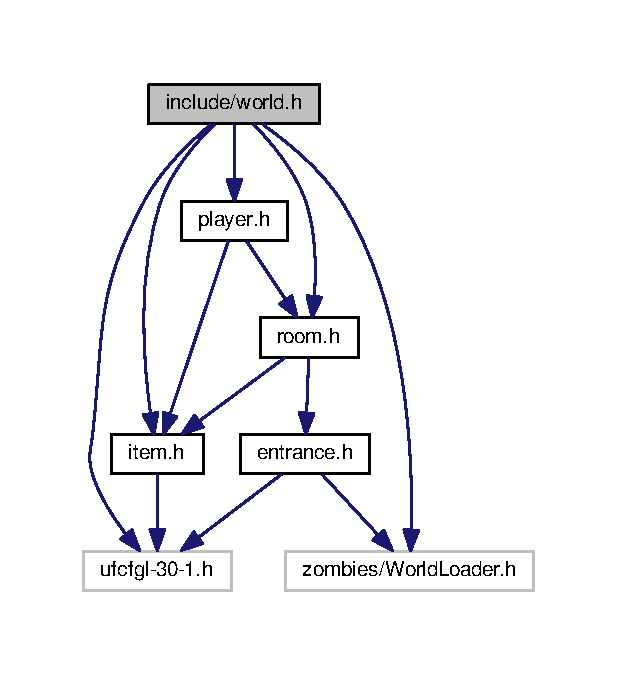
\includegraphics[width=296pt]{world_8h__incl}
\end{center}
\end{figure}
This graph shows which files directly or indirectly include this file\+:
\nopagebreak
\begin{figure}[H]
\begin{center}
\leavevmode
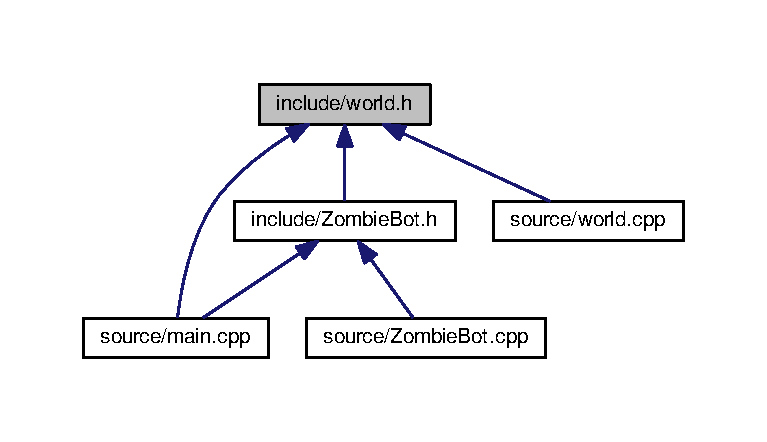
\includegraphics[width=350pt]{world_8h__dep__incl}
\end{center}
\end{figure}
\subsection*{Classes}
\begin{DoxyCompactItemize}
\item 
class \hyperlink{class_world}{World}
\end{DoxyCompactItemize}

\hypertarget{_zombie_bot_8h}{}\section{include/\+Zombie\+Bot.h File Reference}
\label{_zombie_bot_8h}\index{include/\+Zombie\+Bot.\+h@{include/\+Zombie\+Bot.\+h}}
{\ttfamily \#include $<$zombies/\+Zombie\+Bot.\+h$>$}\\*
{\ttfamily \#include \char`\"{}world.\+h\char`\"{}}\\*
Include dependency graph for Zombie\+Bot.\+h\+:
\nopagebreak
\begin{figure}[H]
\begin{center}
\leavevmode
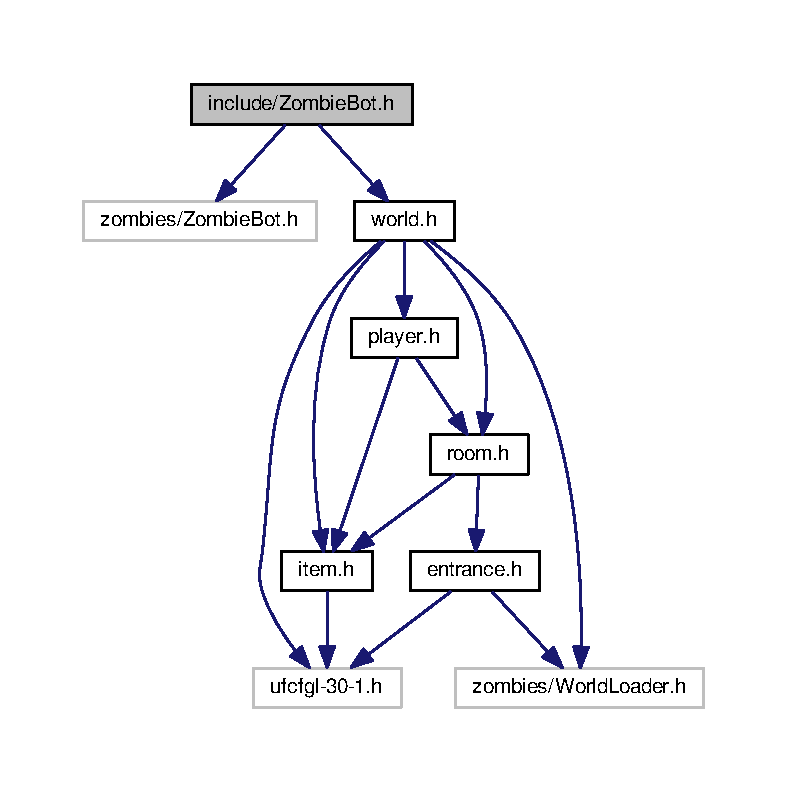
\includegraphics[width=350pt]{_zombie_bot_8h__incl}
\end{center}
\end{figure}
This graph shows which files directly or indirectly include this file\+:
\nopagebreak
\begin{figure}[H]
\begin{center}
\leavevmode
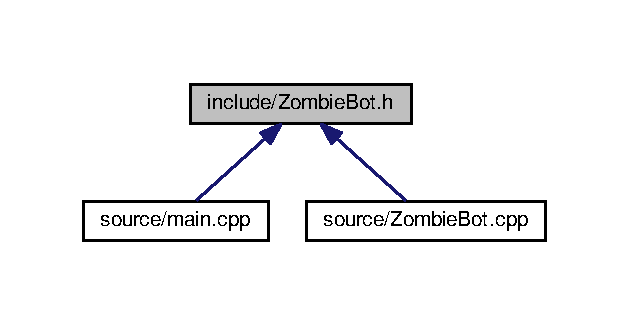
\includegraphics[width=302pt]{_zombie_bot_8h__dep__incl}
\end{center}
\end{figure}
\subsection*{Classes}
\begin{DoxyCompactItemize}
\item 
class \hyperlink{class_zombie_bot}{Zombie\+Bot}
\end{DoxyCompactItemize}

\hypertarget{entrance_8cpp}{}\section{source/entrance.cpp File Reference}
\label{entrance_8cpp}\index{source/entrance.\+cpp@{source/entrance.\+cpp}}
{\ttfamily \#include \char`\"{}entrance.\+h\char`\"{}}\\*
Include dependency graph for entrance.\+cpp\+:
\nopagebreak
\begin{figure}[H]
\begin{center}
\leavevmode
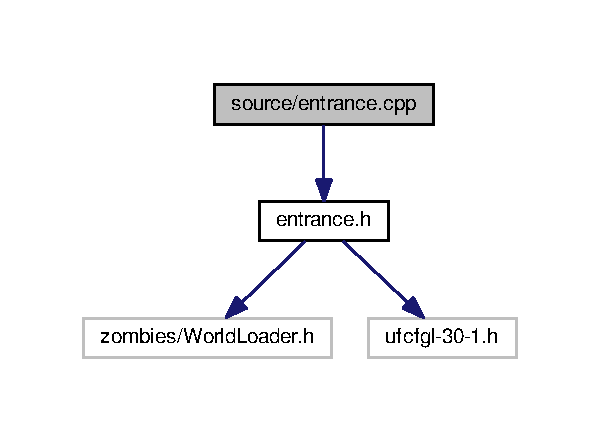
\includegraphics[width=288pt]{entrance_8cpp__incl}
\end{center}
\end{figure}

\hypertarget{item_8cpp}{}\section{source/item.cpp File Reference}
\label{item_8cpp}\index{source/item.\+cpp@{source/item.\+cpp}}
{\ttfamily \#include \char`\"{}item.\+h\char`\"{}}\\*
Include dependency graph for item.\+cpp\+:
\nopagebreak
\begin{figure}[H]
\begin{center}
\leavevmode
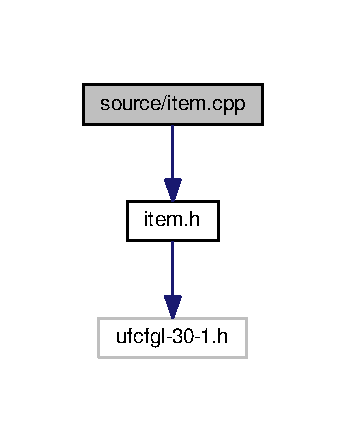
\includegraphics[width=166pt]{item_8cpp__incl}
\end{center}
\end{figure}

\hypertarget{main_8cpp}{}\section{source/main.cpp File Reference}
\label{main_8cpp}\index{source/main.\+cpp@{source/main.\+cpp}}
{\ttfamily \#include $<$ufcfgl-\/30-\/1.\+h$>$}\\*
{\ttfamily \#include $<$zombies/\+World\+Loader.\+h$>$}\\*
{\ttfamily \#include $<$zombies/\+Zombie\+Server.\+h$>$}\\*
{\ttfamily \#include \char`\"{}Zombie\+Bot.\+h\char`\"{}}\\*
{\ttfamily \#include \char`\"{}world.\+h\char`\"{}}\\*
Include dependency graph for main.\+cpp\+:
\nopagebreak
\begin{figure}[H]
\begin{center}
\leavevmode
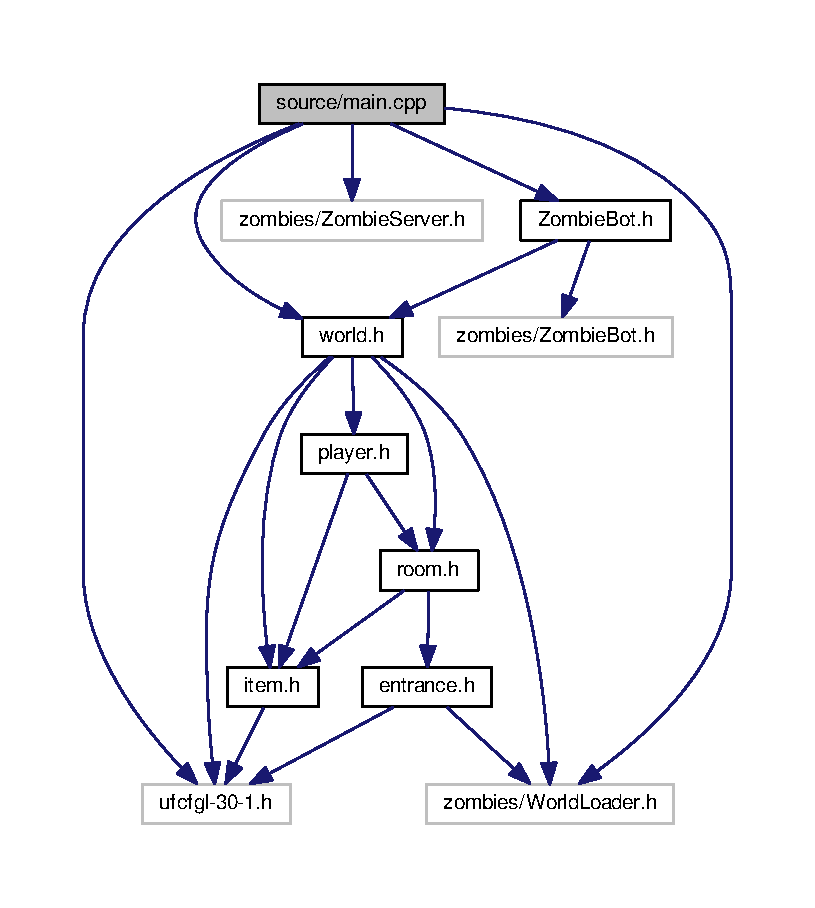
\includegraphics[width=350pt]{main_8cpp__incl}
\end{center}
\end{figure}
\subsection*{Functions}
\begin{DoxyCompactItemize}
\item 
int \hyperlink{main_8cpp_a840291bc02cba5474a4cb46a9b9566fe}{main} (void)
\end{DoxyCompactItemize}


\subsection{Function Documentation}
\index{main.\+cpp@{main.\+cpp}!main@{main}}
\index{main@{main}!main.\+cpp@{main.\+cpp}}
\subsubsection[{\texorpdfstring{main(void)}{main(void)}}]{\setlength{\rightskip}{0pt plus 5cm}int main (
\begin{DoxyParamCaption}
\item[{void}]{}
\end{DoxyParamCaption}
)}\hypertarget{main_8cpp_a840291bc02cba5474a4cb46a9b9566fe}{}\label{main_8cpp_a840291bc02cba5474a4cb46a9b9566fe}

\hypertarget{player_8cpp}{}\section{source/player.cpp File Reference}
\label{player_8cpp}\index{source/player.\+cpp@{source/player.\+cpp}}
{\ttfamily \#include \char`\"{}player.\+h\char`\"{}}\\*
Include dependency graph for player.\+cpp\+:
\nopagebreak
\begin{figure}[H]
\begin{center}
\leavevmode
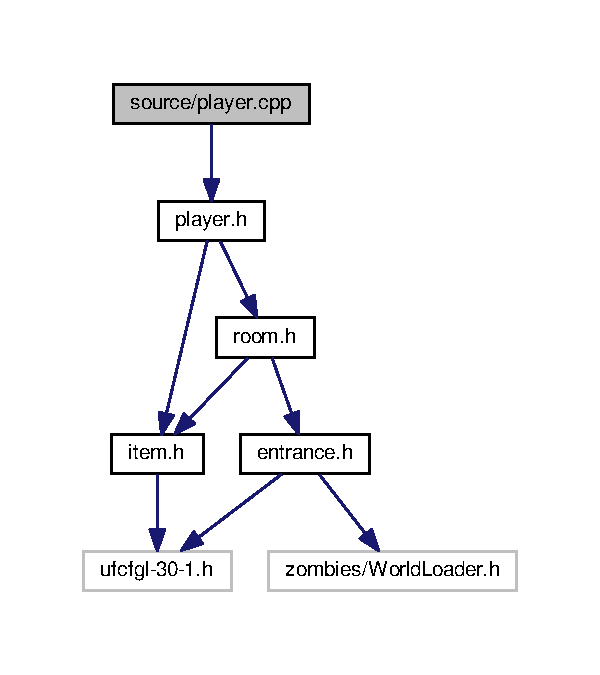
\includegraphics[width=288pt]{player_8cpp__incl}
\end{center}
\end{figure}

\hypertarget{room_8cpp}{}\section{source/room.cpp File Reference}
\label{room_8cpp}\index{source/room.\+cpp@{source/room.\+cpp}}
{\ttfamily \#include \char`\"{}room.\+h\char`\"{}}\\*
{\ttfamily \#include \char`\"{}entrance.\+h\char`\"{}}\\*
Include dependency graph for room.\+cpp\+:
\nopagebreak
\begin{figure}[H]
\begin{center}
\leavevmode
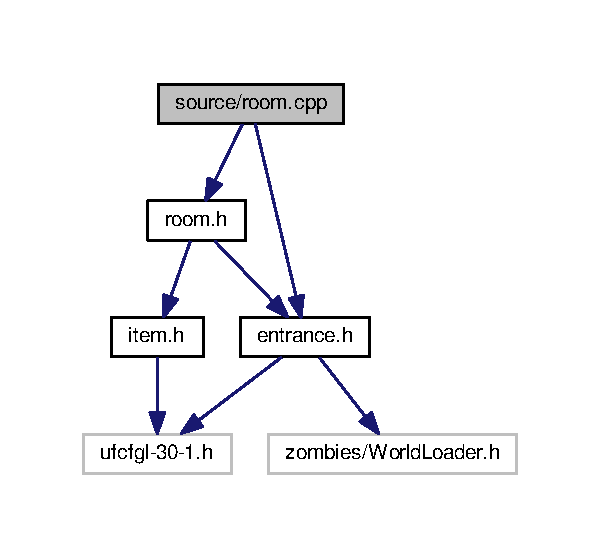
\includegraphics[width=288pt]{room_8cpp__incl}
\end{center}
\end{figure}

\hypertarget{world_8cpp}{}\section{source/world.cpp File Reference}
\label{world_8cpp}\index{source/world.\+cpp@{source/world.\+cpp}}
{\ttfamily \#include \char`\"{}world.\+h\char`\"{}}\\*
Include dependency graph for world.\+cpp\+:
\nopagebreak
\begin{figure}[H]
\begin{center}
\leavevmode
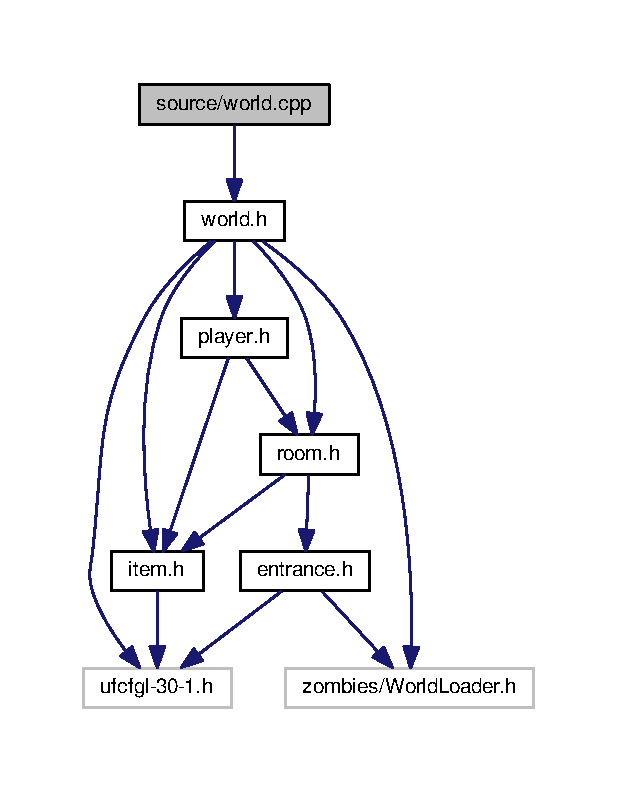
\includegraphics[width=296pt]{world_8cpp__incl}
\end{center}
\end{figure}

\hypertarget{_zombie_bot_8cpp}{}\section{source/\+Zombie\+Bot.cpp File Reference}
\label{_zombie_bot_8cpp}\index{source/\+Zombie\+Bot.\+cpp@{source/\+Zombie\+Bot.\+cpp}}
{\ttfamily \#include $<$iostream$>$}\\*
{\ttfamily \#include $<$sstream$>$}\\*
{\ttfamily \#include $<$algorithm$>$}\\*
{\ttfamily \#include $<$iterator$>$}\\*
{\ttfamily \#include $<$utility$>$}\\*
{\ttfamily \#include $<$ufcfgl-\/30-\/1.\+h$>$}\\*
{\ttfamily \#include \char`\"{}Zombie\+Bot.\+h\char`\"{}}\\*
Include dependency graph for Zombie\+Bot.\+cpp\+:
\nopagebreak
\begin{figure}[H]
\begin{center}
\leavevmode
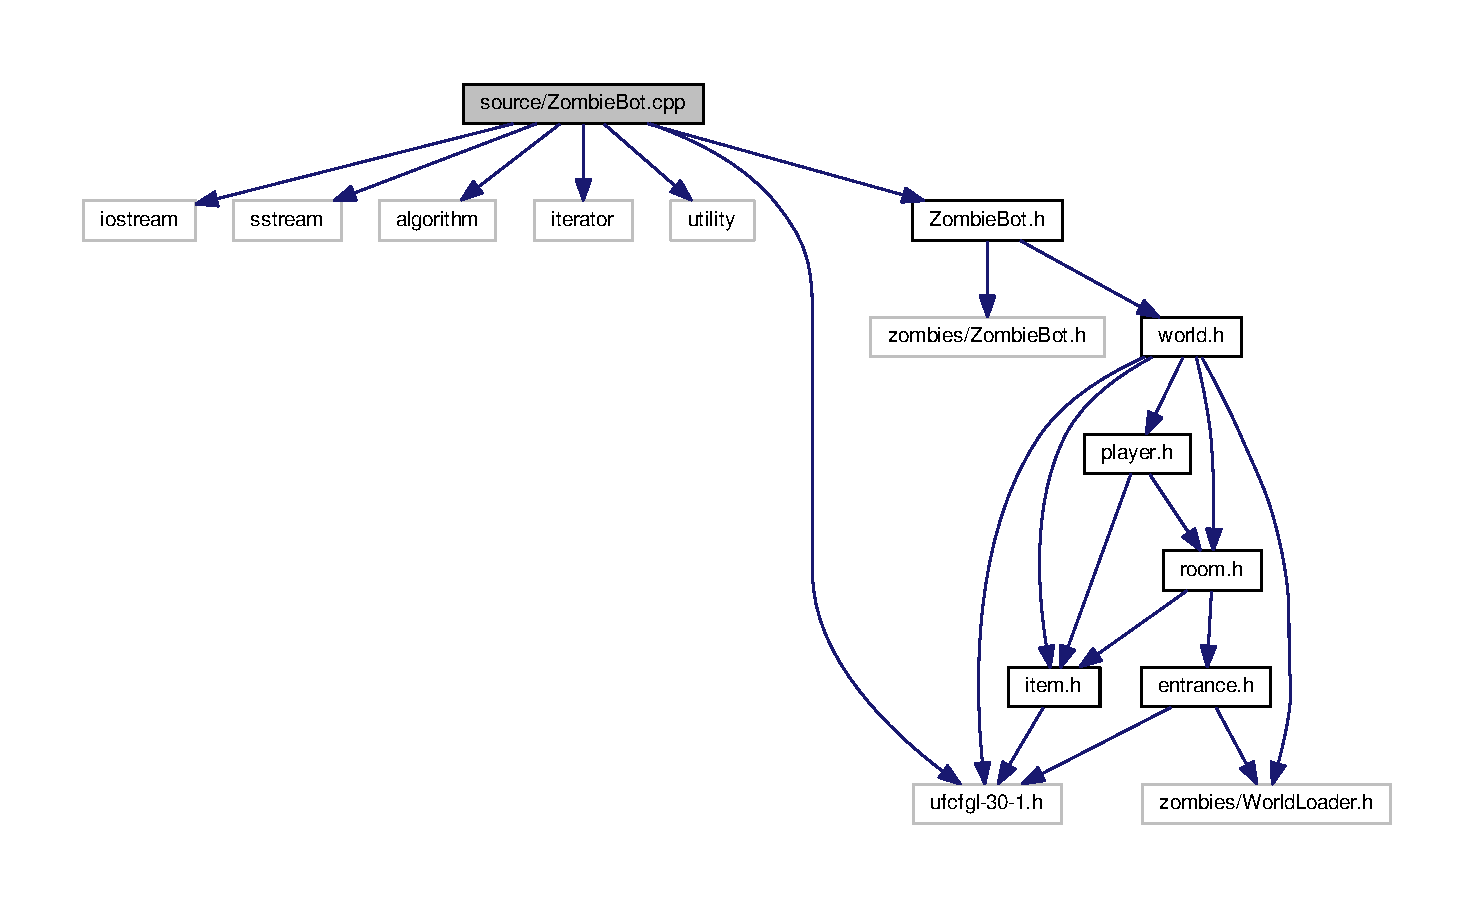
\includegraphics[width=350pt]{_zombie_bot_8cpp__incl}
\end{center}
\end{figure}

%--- End generated contents ---

% Index
\backmatter
\newpage
\phantomsection
\clearemptydoublepage
\addcontentsline{toc}{chapter}{Index}
\printindex

\end{document}
